\documentclass[11pt,oneside]{book}
\usepackage[T1]{fontenc}
\usepackage[utf8]{inputenc}
\usepackage{lmodern}
\usepackage[margin=0.82in,headheight=15pt]{geometry}
\usepackage{microtype}
\usepackage{amsmath,amssymb,amsthm,mathtools}
\usepackage{bm}
\usepackage{graphicx}
\usepackage{booktabs,longtable,tabularx,array,multirow}
\usepackage{enumitem}
\usepackage{xcolor}
\usepackage{caption}
\usepackage{subcaption}
\usepackage{float}
\usepackage[section]{placeins}
\usepackage{fancyhdr}
\usepackage{hyperref}
\usepackage[nameinlink,noabbrev]{cleveref}
\usepackage[most]{tcolorbox}
\usepackage{listings}
\usepackage{url}

\definecolor{ink}{HTML}{17202A}
\definecolor{blue}{HTML}{2E86AB}
\definecolor{teal}{HTML}{2A9D8F}
\definecolor{orange}{HTML}{F4A261}
\definecolor{red}{HTML}{E76F51}
\definecolor{purple}{HTML}{6C5CE7}
\definecolor{paper}{HTML}{FBFBF8}
\definecolor{softgray}{HTML}{EEF1F3}

\hypersetup{
  colorlinks=true,
  linkcolor=purple,
  citecolor=teal,
  urlcolor=blue,
  pdftitle={Projector-Resolved Hodge Calculus I},
  pdfauthor={Komorebi P.},
  pdfsubject={Hodge conjecture decomposition, cycle frames, polyphase refinement, and correspondence reconstruction},
  pdfkeywords={Hodge conjecture, algebraic cycles, projector calculus, polyphase refinement, correspondences}
}

\graphicspath{{figures/}}
\captionsetup{font=small,labelfont=bf,margin=0.04\textwidth}
\setlength{\parindent}{0pt}
\setlength{\parskip}{0.55em}
\setlist[itemize]{leftmargin=1.45em,itemsep=0.25em,topsep=0.3em}
\setlist[enumerate]{leftmargin=1.65em,itemsep=0.25em,topsep=0.3em}
\renewcommand{\arraystretch}{1.16}

\pagestyle{fancy}
\fancyhf{}
\fancyhead[L]{\small Projector-Resolved Hodge Calculus I}
\fancyhead[R]{\small Komorebi P.}
\fancyfoot[C]{\thepage}

\newtheorem{theorem}{Theorem}[chapter]
\newtheorem{proposition}[theorem]{Proposition}
\newtheorem{lemma}[theorem]{Lemma}
\newtheorem{corollary}[theorem]{Corollary}
\theoremstyle{definition}
\newtheorem{definition}[theorem]{Definition}
\newtheorem{construction}[theorem]{Construction}
\newtheorem{problem}[theorem]{Problem}
\theoremstyle{remark}
\newtheorem{remark}[theorem]{Remark}

\newtcolorbox{claimboundary}{
  colback=red!5,colframe=red!75!black,title=Claim boundary,
  fonttitle=\bfseries,breakable,boxrule=0.9pt,arc=1.2mm}
\newtcolorbox{resultbox}[1][]{
  colback=teal!5,colframe=teal!75!black,title={#1},
  fonttitle=\bfseries,breakable,boxrule=0.9pt,arc=1.2mm}
\newtcolorbox{openproblem}[1][]{
  colback=orange!7,colframe=orange!85!black,title={#1},
  fonttitle=\bfseries,breakable,boxrule=0.9pt,arc=1.2mm}
\newtcolorbox{methodbox}[1][]{
  colback=blue!5,colframe=blue!75!black,title={#1},
  fonttitle=\bfseries,breakable,boxrule=0.9pt,arc=1.2mm}

\newcommand{\Hdg}{\operatorname{Hdg}}
\newcommand{\Alg}{\operatorname{Alg}}
\newcommand{\cl}{\operatorname{cl}}
\newcommand{\CH}{\operatorname{CH}}
\newcommand{\im}{\operatorname{im}}
\newcommand{\rank}{\operatorname{rank}}
\newcommand{\Hom}{\operatorname{Hom}}
\newcommand{\End}{\operatorname{End}}
\newcommand{\Tr}{\operatorname{Tr}}
\newcommand{\Span}{\operatorname{span}}
\newcommand{\Q}{\mathbf{Q}}
\newcommand{\R}{\mathbf{R}}
\newcommand{\C}{\mathbf{C}}
\newcommand{\id}{\mathrm{id}}

\newcommand{\compactpart}[1]{%
  \par\vspace{1.2em}\noindent
  \begin{tcolorbox}[colback=purple!5,colframe=purple!70!black,boxrule=0.9pt,arc=1.2mm,left=4mm,right=4mm,top=3mm,bottom=3mm]
  {\Large\bfseries #1}
  \end{tcolorbox}
  \addcontentsline{toc}{part}{#1}
  \markboth{#1}{#1}
  \vspace{0.4em}
}

\lstset{
  basicstyle=\ttfamily\footnotesize,
  frame=single,
  breaklines=true,
  backgroundcolor=\color{softgray},
  rulecolor=\color{softgray},
  showstringspaces=false,
  columns=fullflexible
}

\begin{document}

\frontmatter
\hypersetup{pageanchor=false}
\begin{titlepage}
\centering
\vspace*{0.45in}
{\Huge\bfseries Projector-Resolved Hodge Calculus I\par}
\vspace{0.18in}
{\Large Primitive Hodge Packets, Algebraic Cycle Frames,\par}
{\Large Polyphase Correspondences, and Divisor-Lowering Reconstruction\par}
\vspace{0.32in}
{\large Komorebi P.\par}
\vspace{0.24in}
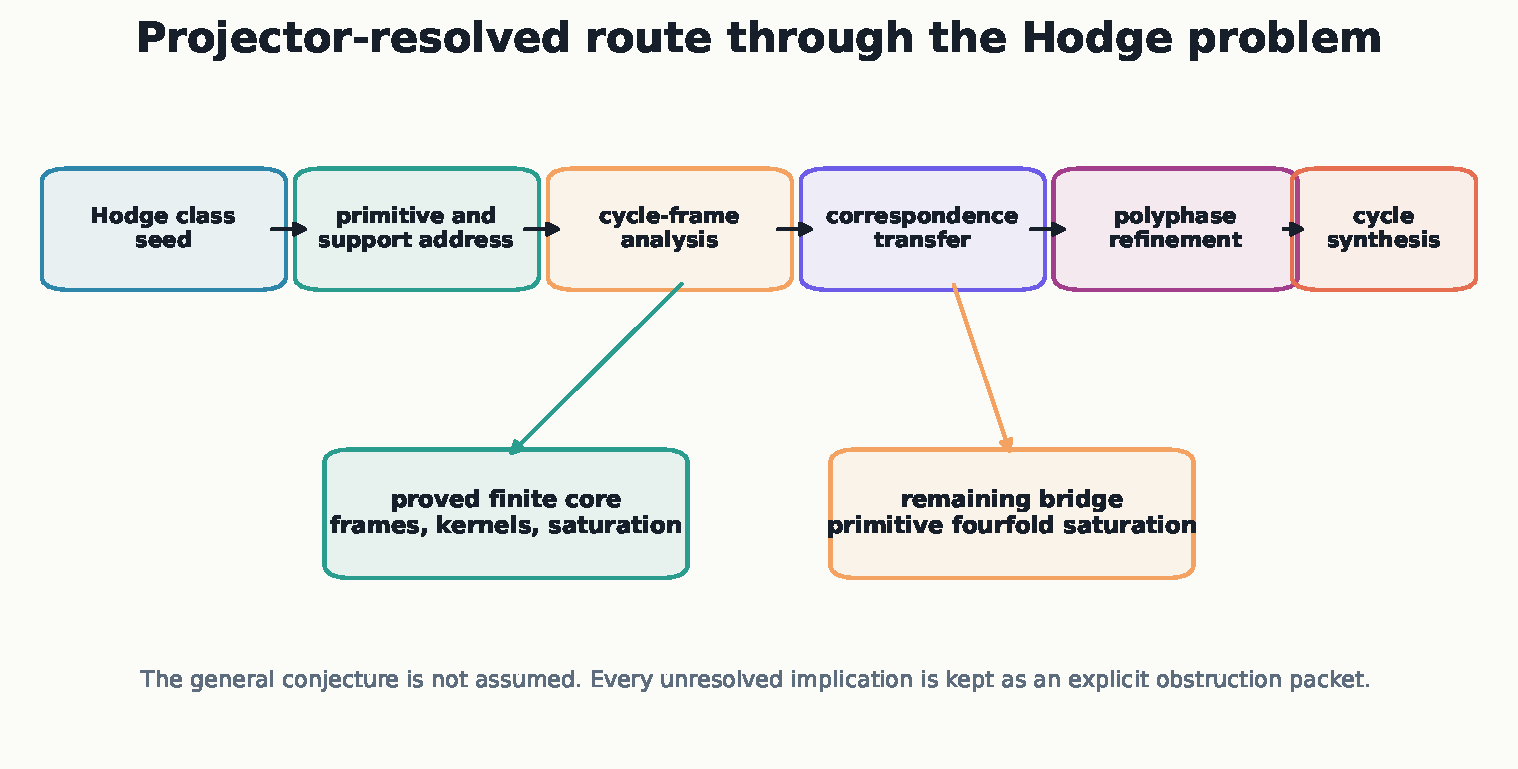
\includegraphics[width=0.82\textwidth]{01_hodge_program_pipeline.pdf}
\vfill
{\small A theorem-by-theorem reconstruction of the Hodge program developed from the projector-resolved seed calculus.\par}
{\small The general rational Hodge conjecture is not claimed as proved.\par}
\vspace{0.15in}
{\small August 2026\par}
\end{titlepage}
\hypersetup{pageanchor=true}

\chapter*{Abstract}
\addcontentsline{toc}{chapter}{Abstract}
This monograph organizes a projector-resolved attack on the rational Hodge conjecture into exact finite statements, classical validation cases, conditional analytic mechanisms, and a sharply isolated open target. The central objects are the rational Hodge projector, the algebraic-cycle projector, positive cycle-frame operators, exact degree-residue polyphase refinements, coniveau support packets, divisor-lowering correspondence channels, Adams degree projectors, and nonlinear Dolbeault obstruction packets. The finite core proves exact reconstruction, positive frame saturation, parent-child assembly, finite stabilization of bounded-degree cycle spans, support verification, rational multiplicity recovery, invertible correspondence reconstruction, and propagation through several geometric operations. Classical cubic fourfold and Gushel-Mukai incidence constructions are used as validation cases rather than claimed as new proofs. The remaining general difficulty is concentrated in primitive middle cohomology, beginning with primitive rational $(2,2)$ classes on projective fourfolds. The proposed next theorem is a multi-incidence saturation result in which line, conic, plane, and exceptional channels jointly detect every primitive Hodge direction even when no individual channel is complete.

\begin{claimboundary}
The general rational Hodge conjecture remains open. This manuscript proves a collection of exact reduction, reconstruction, positivity, and correspondence theorems. It does not prove that every primitive rational Hodge class enters an algebraic cycle channel. Any classical family already covered by established incidence theorems is labeled as validation rather than historical novelty.
\end{claimboundary}

\chapter*{Executive map}
\addcontentsline{toc}{chapter}{Executive map}
The working grammar is
\[
\text{seed}\to\text{address}\to\text{operate}\to\text{project}
\to\text{transfer}\to\text{refine}\to\text{constrain}
\to\text{complete}\to\text{reconstruct}.
\]
For the Hodge problem, the seed is a rational cohomology class. Its first address is Hodge type, followed by Lefschetz depth, algebraic support, cycle degree, symmetry character, and arithmetic phase. Analysis is performed by cycle classes or algebraic correspondences. Refinement replaces one parent channel by complete children while preserving the total positive frame operator. The unresolved class is the intersection of the kernels of all available analysis channels.

\begin{center}
\begin{tabular}{p{0.23\textwidth}p{0.23\textwidth}p{0.42\textwidth}}
\toprule
Layer & Main object & Exact question \\
\midrule
Hodge selection & $P_{\Hdg}^p$ & Is the rational $(p,p)$ packet nonzero? \\
Algebraic selection & $P_{\Alg}^p$ & Which directions are already generated by cycles? \\
Master obstruction & $\mathcal O_X^p=P_{\Hdg}^p-P_{\Alg}^p$ & Does any Hodge direction survive all algebraic channels? \\
Cycle frame & $S_D=C_DC_D^*$ & Does a finite cycle family span the Hodge packet? \\
Polyphase refinement & $S_{M,r}=\sum_j S_{LM,r+jM}$ & Can separate geometric methods solve separate children? \\
Correspondence transfer & $T=\sum_rB_rA_r$ & Is lowering to divisor degree and returning invertible? \\
Analytic obstruction & $\Phi_A$ & Does the finite nonlinear obstruction packet vanish? \\
\bottomrule
\end{tabular}
\end{center}

{\small\setlength{\parskip}{0pt}\tableofcontents}

\mainmatter

\addcontentsline{toc}{part}{Part I. The conjecture as a projector problem}

\chapter{The rational Hodge target}
\section{Statement and status}
Let $X$ be a smooth projective complex variety. For each codimension $p$, define
\[
\Hdg^p(X)=H^{2p}(X,\Q)\cap H^{p,p}(X)
\]
and
\[
\Alg^p(X)=\im\bigl(\CH^p(X)_{\Q}\xrightarrow{\cl}H^{2p}(X,\Q)\bigr).
\]
Every algebraic cycle class has type $(p,p)$, so $\Alg^p(X)\subseteq\Hdg^p(X)$. The rational Hodge conjecture asserts equality for every smooth projective $X$ and every $p$ \cite{ClayHodge,VoisinHodge}.

Choose a polarization-compatible positive inner product on $H^{2p}(X,\R)$ and let $P_{\Hdg}^p$ and $P_{\Alg}^p$ denote orthogonal projectors. Since the algebraic space is nested in the Hodge space,
\[
P_{\Hdg}^pP_{\Alg}^p=P_{\Alg}^p.
\]

\begin{proposition}[Master obstruction projector]
The operator
\[
\mathcal O_X^p=P_{\Hdg}^p-P_{\Alg}^p
\]
is the orthogonal projector onto $\Hdg^p(X)\cap\Alg^p(X)^\perp$. Therefore
\[
\mathcal O_X^p=0
\quad\Longleftrightarrow\quad
\Hdg^p(X)=\Alg^p(X).
\]
\end{proposition}
\begin{proof}
For nested orthogonal projectors $Q\le P$, the difference $P-Q$ is self-adjoint and
\[
(P-Q)^2=P-PQ-QP+Q=P-Q.
\]
Its range is $\im P\cap(\im Q)^\perp$.
\end{proof}

\begin{figure}[htbp]
\centering
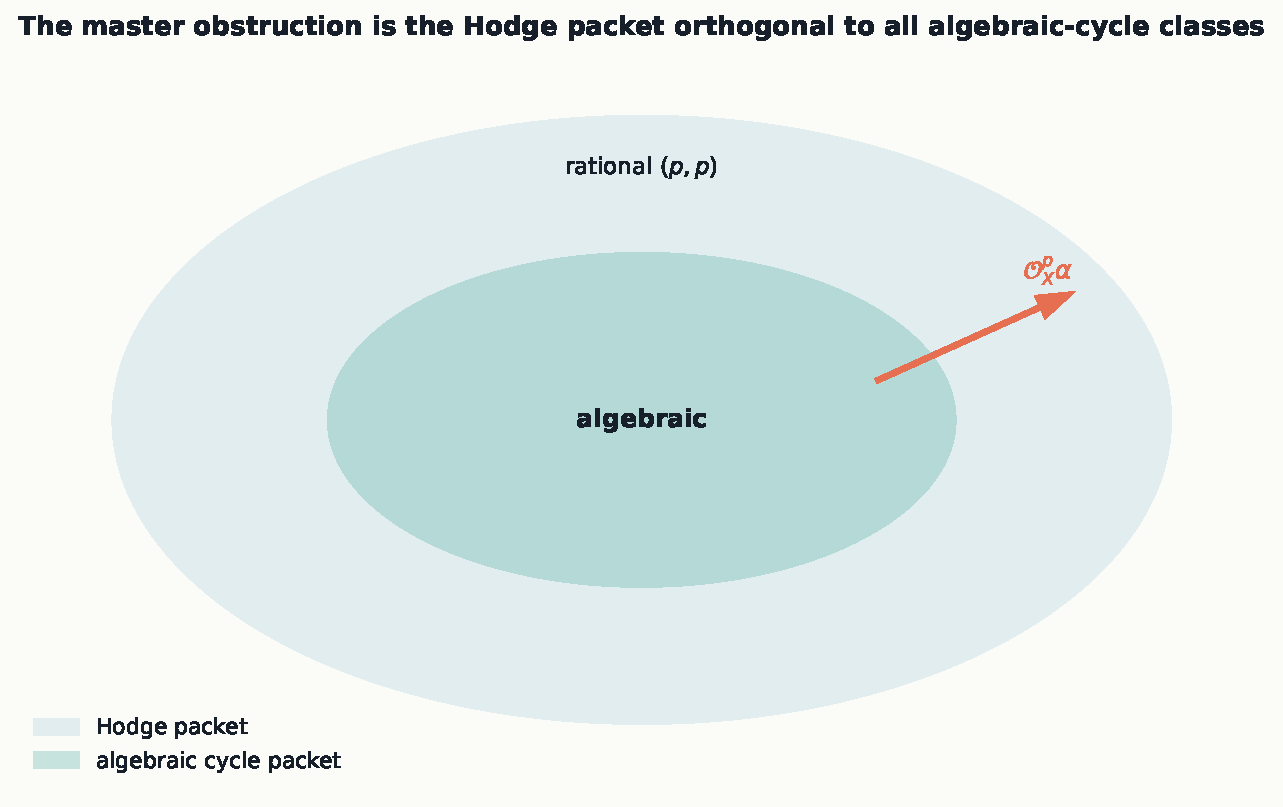
\includegraphics[width=0.82\textwidth]{04_master_obstruction_projector.pdf}
\caption{The master obstruction packet is the rational Hodge subspace not yet covered by algebraic cycle classes.}
\end{figure}

\section{Why dimension four is the first focused target}
The first general unresolved middle case occurs for primitive degree-four cohomology on a smooth projective fourfold. The Hodge diamond highlights the central packet.

\begin{figure}[htbp]
\centering
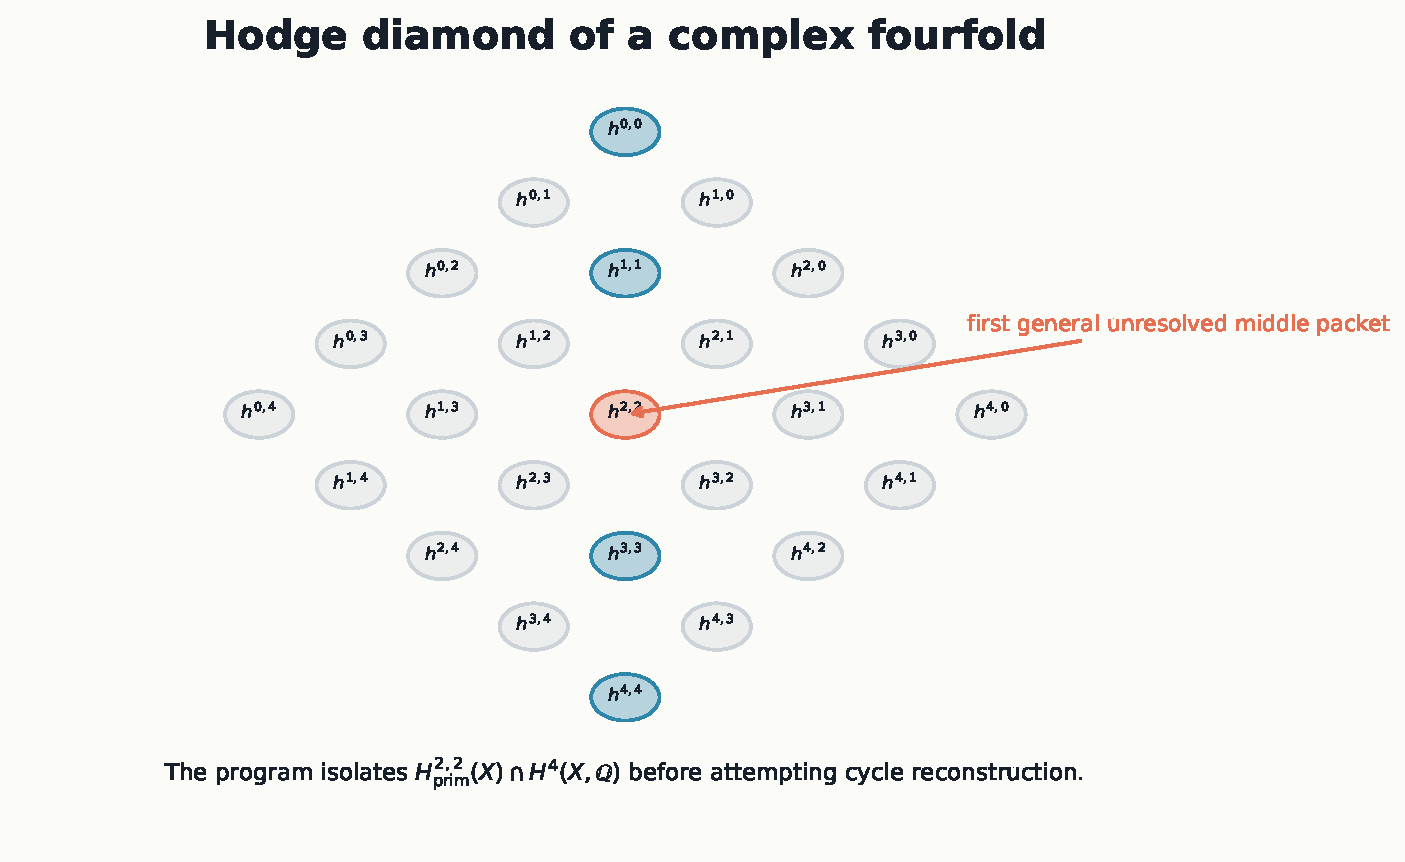
\includegraphics[width=0.68\textwidth]{02_fourfold_hodge_diamond.pdf}
\caption{The primitive rational $(2,2)$ packet in $H^4$ is the first general target retained by the program.}
\end{figure}

\chapter{Primitive and coniveau reductions}
\section{Lefschetz packet decomposition}
Let $h\in H^2(X,\Q)$ be the class of an ample divisor and let $L(\alpha)=h\smile\alpha$. Hard Lefschetz and primitive decomposition yield
\[
H^{2p}(X,\Q)=\bigoplus_{r\ge0}L^rH_{\mathrm{prim}}^{2p-2r}(X,\Q).
\]
The decomposition respects Hodge type.

\begin{theorem}[Primitive reduction]
If every primitive rational Hodge class is algebraic, then every rational Hodge class is algebraic.
\end{theorem}
\begin{proof}
Write $\alpha=\sum_rL^r\alpha_r$ with each $\alpha_r$ primitive and of Hodge type. The class $h$ is algebraic. If $\alpha_r$ is algebraic, then $L^r\alpha_r=h^r\smile\alpha_r$ is algebraic. Summing gives an algebraic representative of $\alpha$.
\end{proof}

For a fourfold and $p=2$,
\[
\alpha=L\beta+\alpha_{\mathrm{prim}},
\qquad
\beta\in H^{1,1}(X)\cap H^2(X,\Q).
\]
The Lefschetz $(1,1)$ theorem makes $\beta$ algebraic. Only $\alpha_{\mathrm{prim}}$ remains.

\begin{figure}[htbp]
\centering
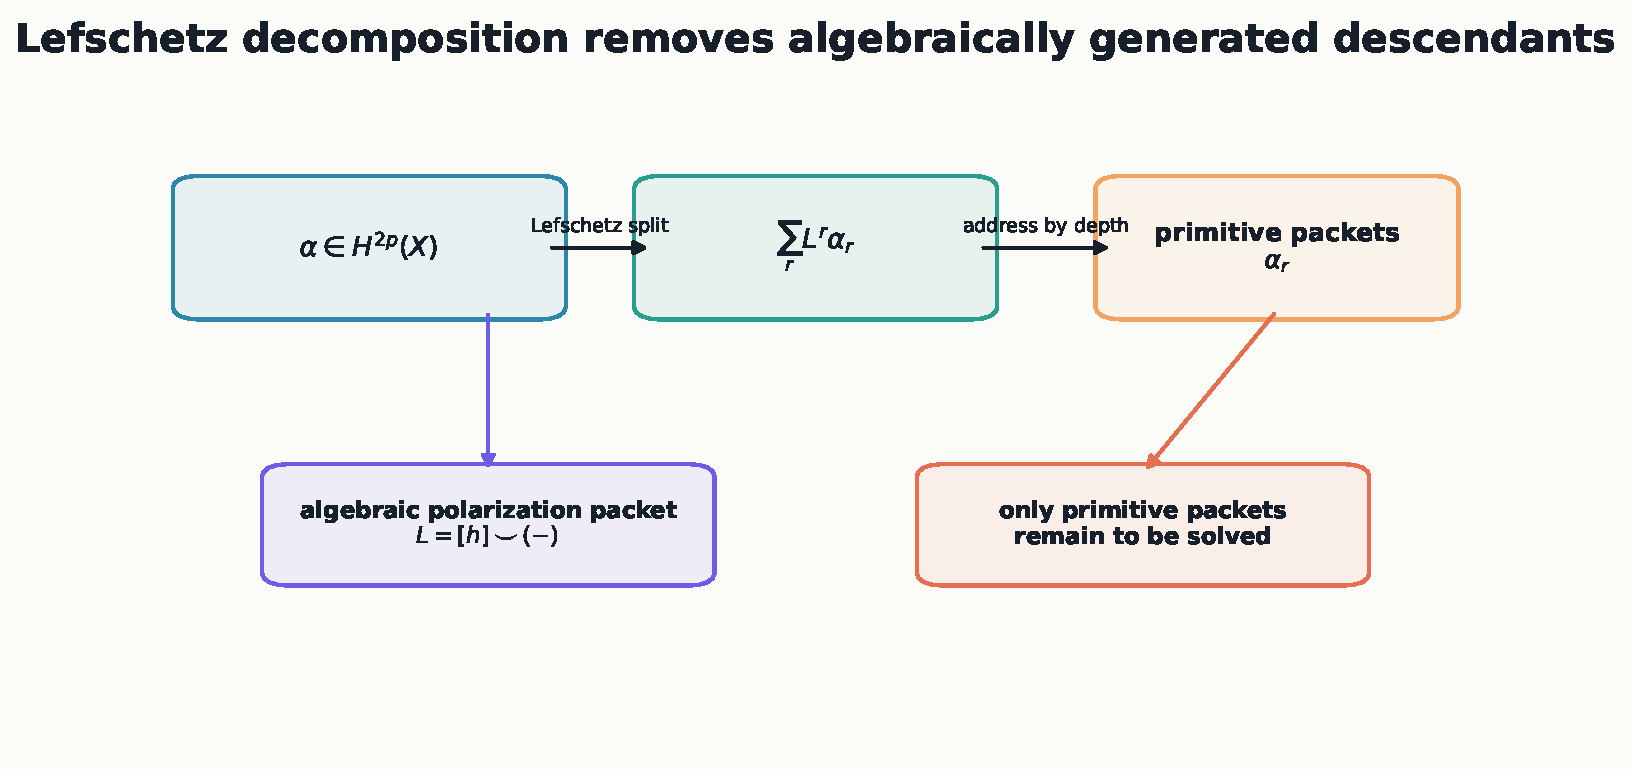
\includegraphics[width=0.82\textwidth]{03_lefschetz_primitive_reduction.pdf}
\caption{Algebraic powers of the polarization remove all Lefschetz descendants, leaving primitive packets.}
\end{figure}

\section{Support localization and coniveau}
Let $N^pH^{2p}(X,\Q)$ be the geometric coniveau-$p$ subspace. In degree $2p$, purity forces support contributions of codimension $p$ to be generated by fundamental classes of codimension-$p$ components.

\begin{theorem}[Degree-$2p$ coniveau identification]
For smooth projective $X$,
\[
N^pH^{2p}(X,\Q)=\Alg^p(X).
\]
\end{theorem}
\begin{proof}[Proof sketch]
The inclusion from right to left is immediate because a codimension-$p$ cycle is supported on its underlying algebraic set. Conversely, a class in coniveau $p$ is in the image of cohomology with supports in an algebraic subset $Z$ of codimension at least $p$. Contributions from components of codimension greater than $p$ vanish in degree $2p$. Purity identifies the degree-$2p$ supported contribution of each codimension-$p$ irreducible component with its fundamental class. Resolution and additivity reduce a general $Z$ to these components.
\end{proof}

Thus the conjecture is equivalently the support statement
\[
\Hdg^p(X)\subseteq N^pH^{2p}(X,\Q).
\]

\begin{figure}[htbp]
\centering
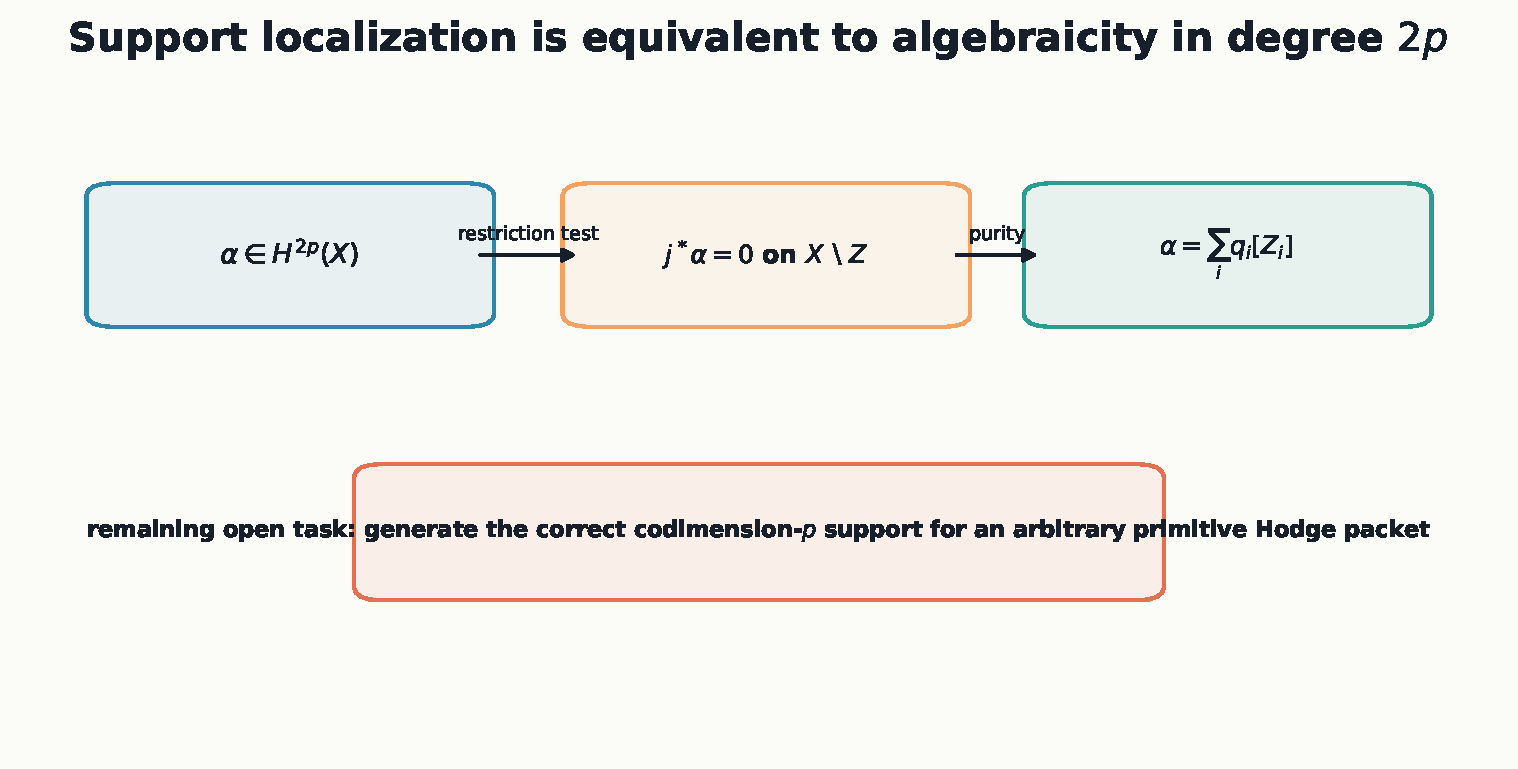
\includegraphics[width=0.84\textwidth]{05_support_localization_pipeline.pdf}
\caption{A verified codimension-$p$ support turns the Hodge class into a finite rational combination of support components.}
\end{figure}

\addcontentsline{toc}{part}{Part II. Algebraic cycle frames and exact polyphase refinement}

\chapter{Positive cycle-frame calculus}
\section{Analysis and synthesis}
Fix a finite family of rational algebraic cycle classes
\[
c_1,\ldots,c_N\in H^{2p}(X,\Q).
\]
Let $V\subseteq H^{2p}(X,\R)$ be the Hodge packet under study. Define
\[
C:\R^N\to H^{2p}(X,\R),
\qquad Ce_j=c_j,
\]
and the positive frame operator
\[
S=CC^*=\sum_{j=1}^N|c_j\rangle\langle c_j|.
\]

\begin{theorem}[Finite positive cycle-frame certificate]
Let $A=\Span_{\R}\{c_1,\ldots,c_N\}$. Then
\[
\im S=A,
\qquad
\ker S=A^\perp.
\]
The selected cycles span $V$ if and only if $S|_V$ is positive definite.
\end{theorem}
\begin{proof}
The equality $\im(CC^*)=\im C$ is standard. Moreover
\[
\langle v,Sv\rangle=\|C^*v\|^2=\sum_j|\langle c_j,v\rangle|^2.
\]
This vanishes exactly when $v$ is orthogonal to every cycle class.
\end{proof}

If $H$ is a matrix whose columns form an orthonormal basis of $V$, the finite Gram certificate is
\[
G=H^*SH.
\]
Then $A\supseteq V$ if and only if $\lambda_{\min}(G)>0$.

\begin{figure}[htbp]
\centering
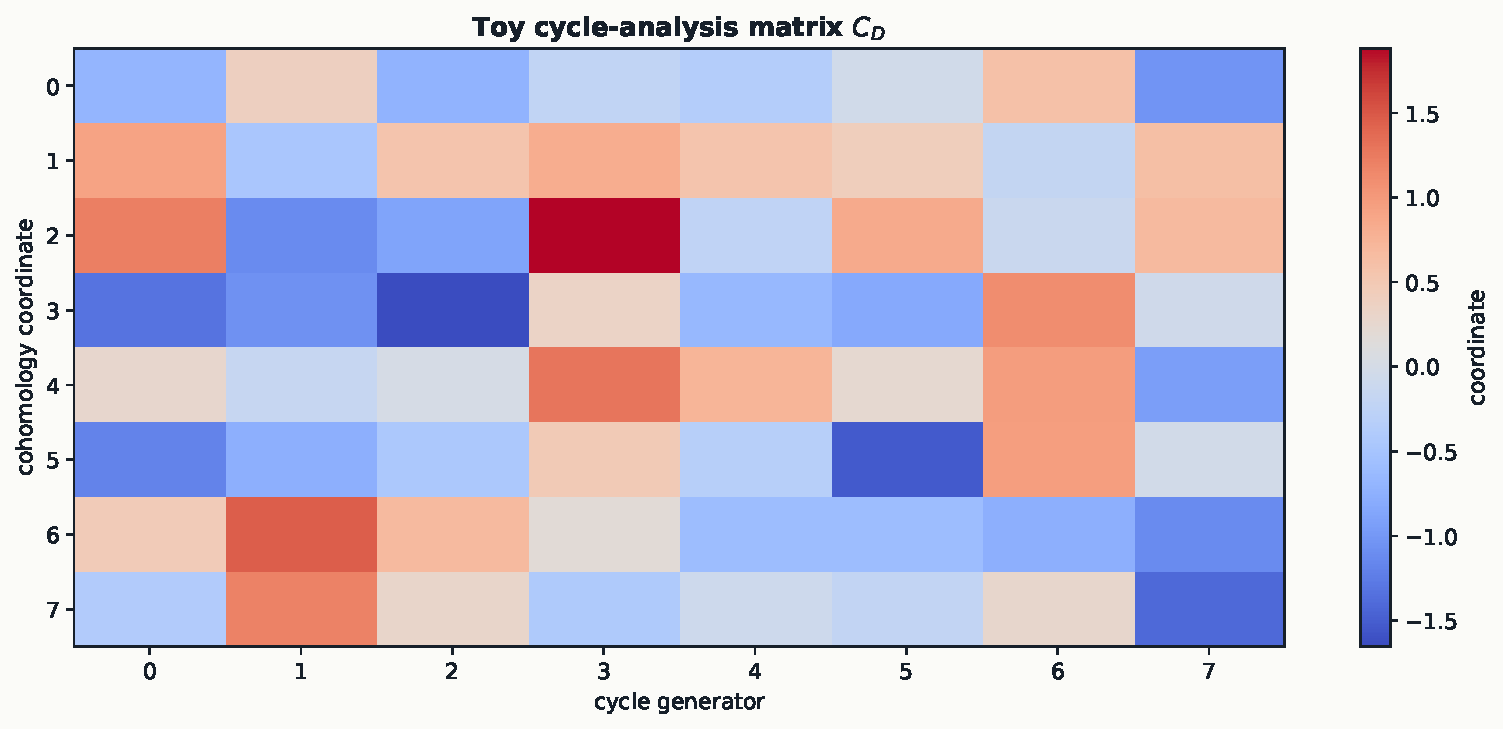
\includegraphics[width=0.82\textwidth]{06_cycle_analysis_matrix.pdf}
\caption{A finite cycle-analysis matrix records cohomology coordinates of candidate algebraic cycles.}
\end{figure}

\begin{figure}[htbp]
\centering
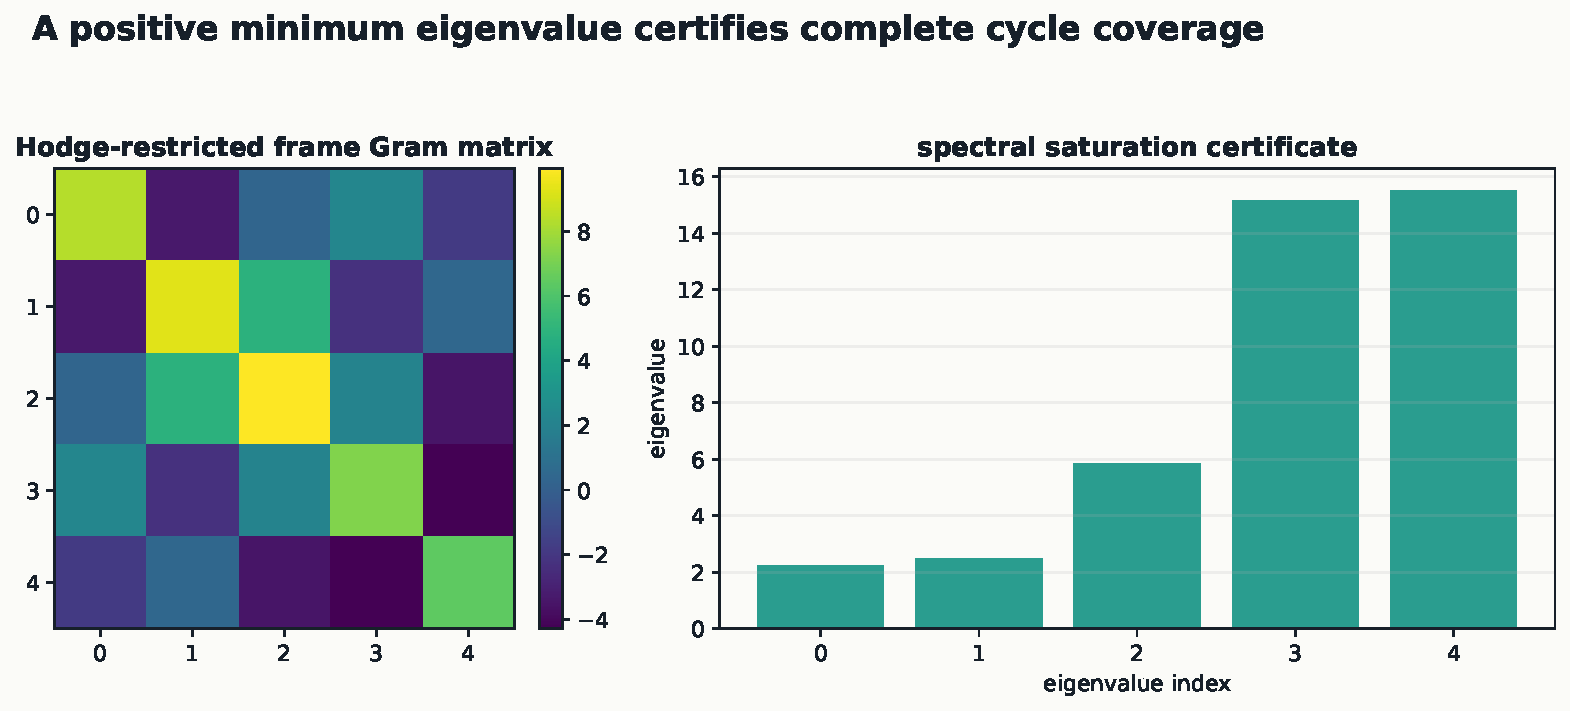
\includegraphics[width=0.9\textwidth]{07_cycle_frame_spectrum.pdf}
\caption{The Hodge-restricted Gram spectrum gives a finite spectral saturation certificate.}
\end{figure}

The orthogonal synthesis of a class $\alpha$ from the cycle span is
\[
P_A\alpha=S S^\dagger\alpha.
\]
If $\alpha\in A$, this is exact.

\begin{figure}[htbp]
\centering
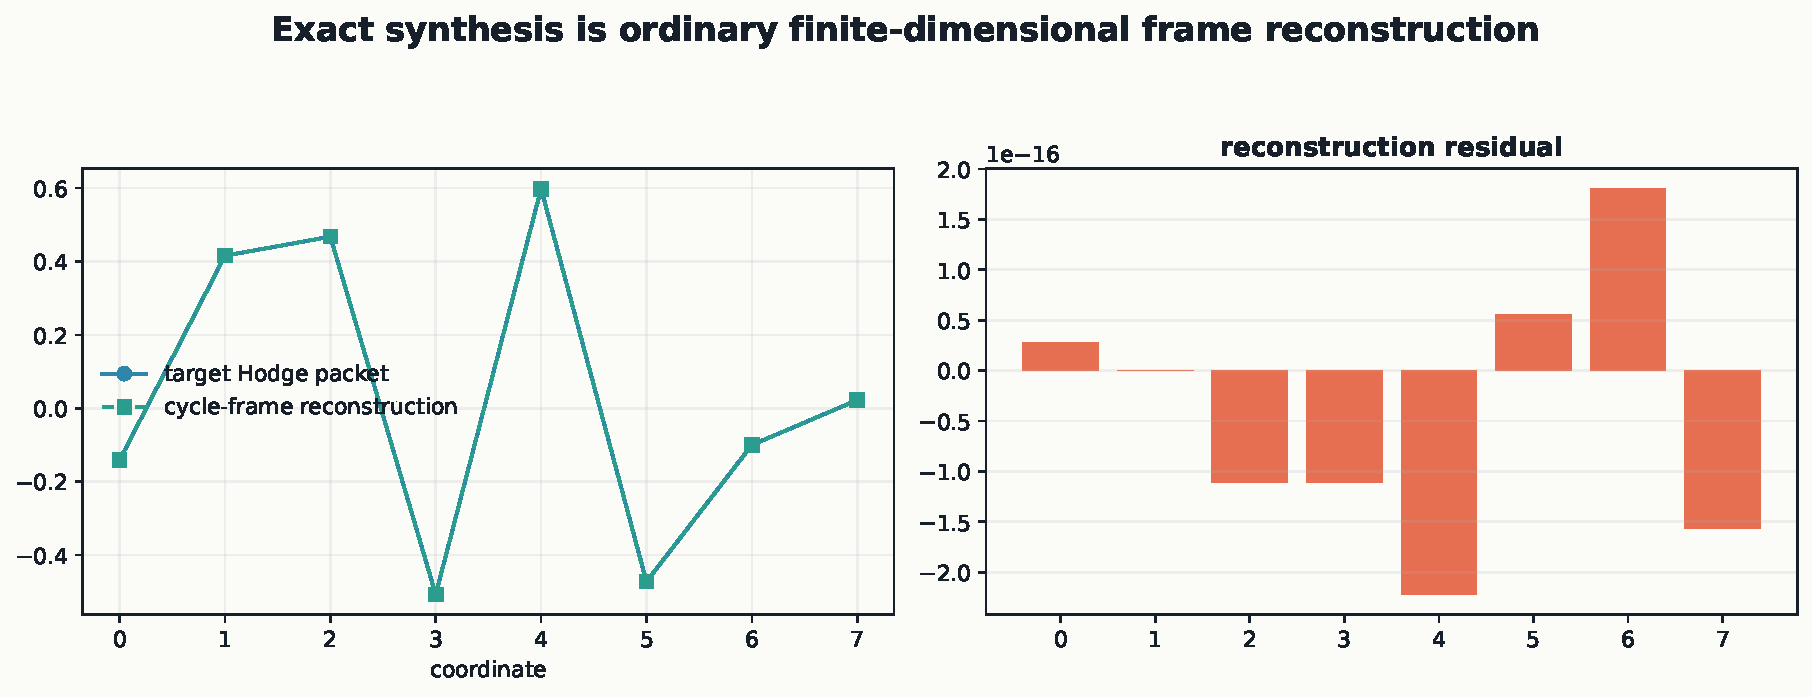
\includegraphics[width=0.88\textwidth]{08_cycle_frame_reconstruction.pdf}
\caption{Finite-dimensional frame synthesis reconstructs the class whenever it lies in the algebraic span.}
\end{figure}

\section{Packet assembly without false orthogonality}
Partition the cycle indices into packets $I_\lambda$. Define
\[
S_\lambda=\sum_{j\in I_\lambda}|c_j\rangle\langle c_j|.
\]
Then
\[
S=\sum_\lambda S_\lambda.
\]
No orthogonality of the child spans is assumed.

\begin{theorem}[Positive child-kernel intersection]
For any subspace $V$,
\[
\ker(S|_V)=\bigcap_\lambda\ker(S_\lambda|_V).
\]
\end{theorem}
\begin{proof}
If $Sv=0$, positivity gives
\[
0=\langle v,Sv\rangle=\sum_\lambda\langle v,S_\lambda v\rangle.
\]
Each nonnegative summand vanishes, which implies $S_\lambda v=0$. The converse is immediate.
\end{proof}

\begin{figure}[htbp]
\centering
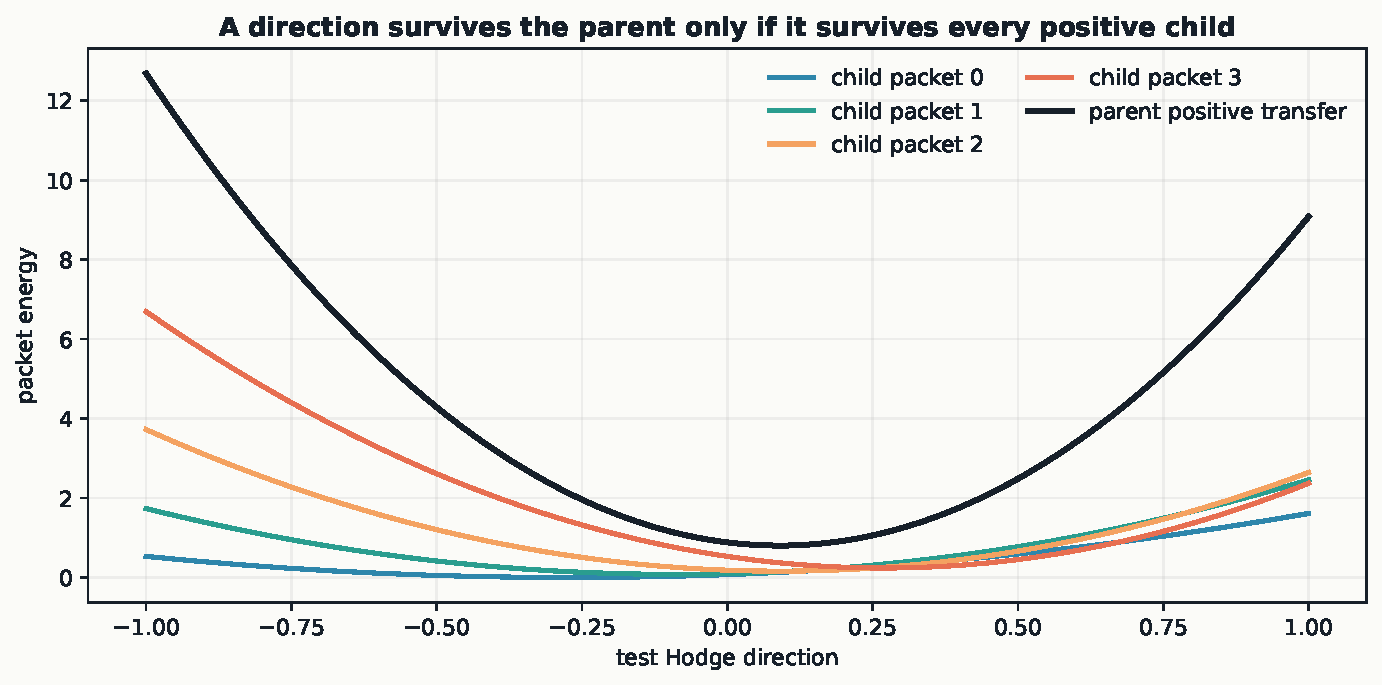
\includegraphics[width=0.84\textwidth]{11_child_kernel_intersection.pdf}
\caption{A Hodge direction survives the parent obstruction only when every positive child channel misses it.}
\end{figure}

\chapter{Degree-residue polyphase refinement}
\section{Exact parent-child frame law}
Fix a projective embedding and assign each cycle its degree. For modulus $M$, define the residue packet
\[
I_{M,r}=\{j:\deg Z_j\equiv r\pmod M\},
\qquad
S_{M,r}=\sum_{j\in I_{M,r}}|c_j\rangle\langle c_j|.
\]

\begin{theorem}[Exact degree polyphase refinement]
For every positive integer $L$,
\[
S_{M,r}=\sum_{\ell=0}^{L-1}S_{LM,r+\ell M}.
\]
\end{theorem}
\begin{proof}
The congruence class $r$ modulo $M$ is the disjoint union of the classes $r+\ell M$ modulo $LM$. The rank-one frame terms are partitioned accordingly.
\end{proof}

\begin{figure}[htbp]
\centering
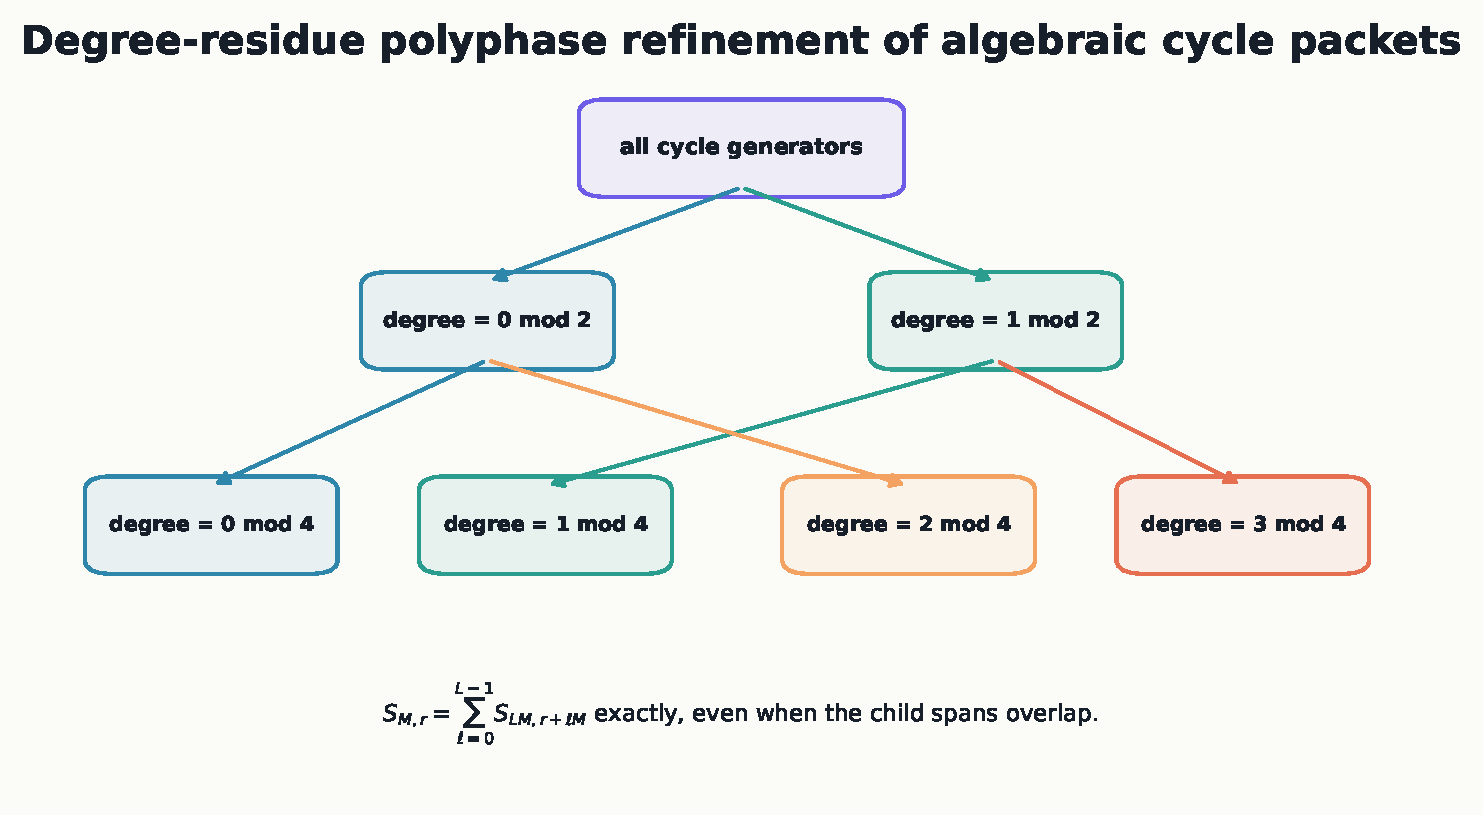
\includegraphics[width=0.82\textwidth]{09_degree_polyphase_tree.pdf}
\caption{Degree addresses refine from modulo $2$ to modulo $4$ while the total cycle frame remains unchanged.}
\end{figure}

\begin{figure}[htbp]
\centering
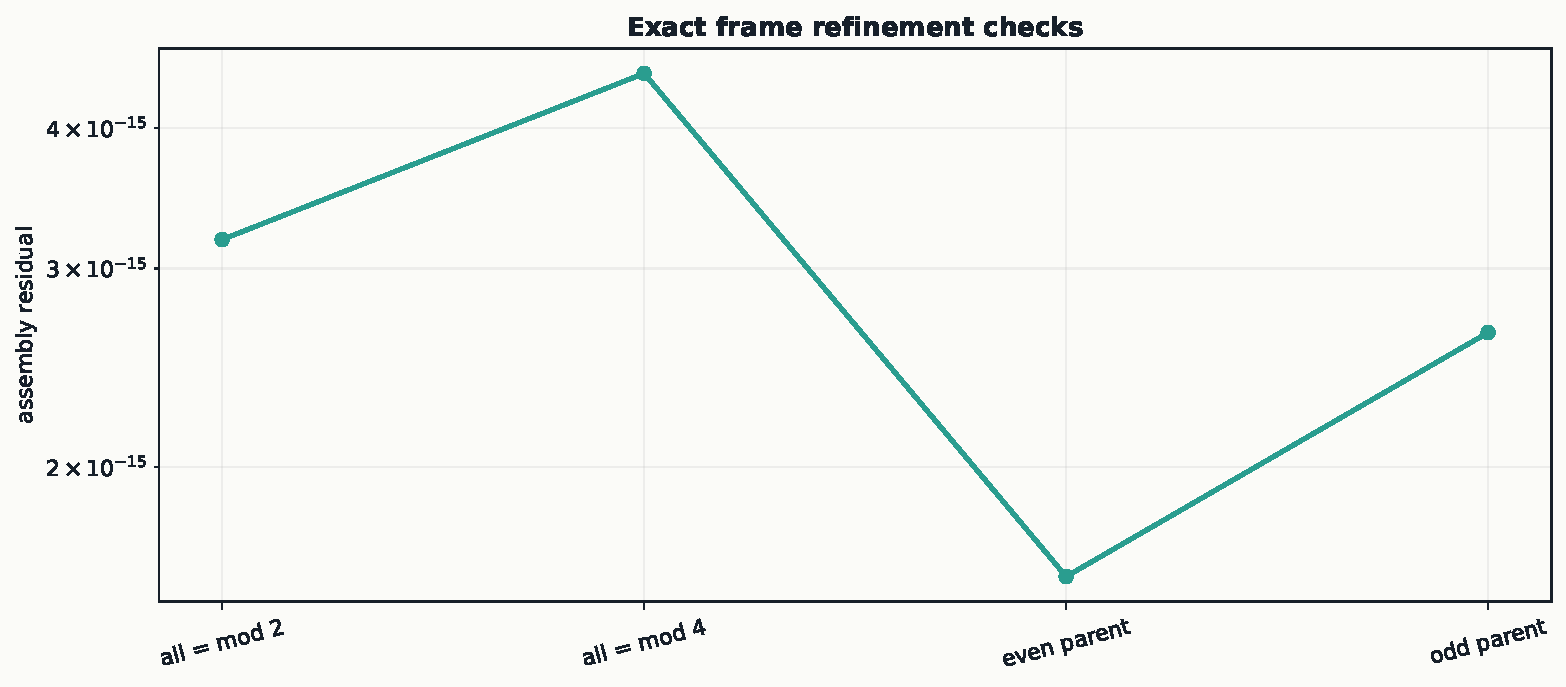
\includegraphics[width=0.76\textwidth]{10_polyphase_assembly_residuals.pdf}
\caption{Numerical certificates of exact parent-child frame assembly in the reproducible toy model.}
\end{figure}

\section{Multiaxial packet addresses}
Degree residue is only one address. A refined cycle packet may be labeled by
\[
\lambda=(r_{\mathrm{Lef}},r_{\deg},\chi_{\mathrm{mon}},s_{\mathrm{supp}},\nu_{\mathrm{Frob}}).
\]
The entries record Lefschetz depth, degree residue, monodromy or symmetry type, support stratum, and arithmetic phase. The total positive frame remains the sum of all leaves. This allows independent methods to solve different geometric sectors before exact synthesis.

\chapter{Finite saturation and exact rational closure}
For each degree cutoff $D$, let $A_D^p(X)$ be the rational span of codimension-$p$ cycle classes of degree at most $D$. Then
\[
A_1^p\subseteq A_2^p\subseteq\cdots\subseteq H^{2p}(X,\Q).
\]

\begin{theorem}[Finite stabilization]
There exists $D_0$ such that $A_D^p(X)=A_{D_0}^p(X)$ for every $D\ge D_0$.
\end{theorem}
\begin{proof}
The dimensions form a nondecreasing sequence of integers bounded by $\dim H^{2p}(X,\Q)$. Only finitely many strict increases are possible.
\end{proof}

\begin{corollary}[Approximation becomes exact]
Let $P_D$ be the orthogonal projector onto $A_D^p(X)\otimes\R$. For a rational class $\alpha$,
\[
\lim_{D\to\infty}\|(I-P_D)\alpha\|=0
\]
if and only if $\alpha\in A_D^p(X)$ for some finite $D$.
\end{corollary}
\begin{proof}
After stabilization, the residual is constant. A constant tail converging to zero is zero.
\end{proof}

Because the matrices and target vector can be chosen over $\Q$, real membership implies rational membership by row reduction over $\Q$.

\begin{figure}[htbp]
\centering
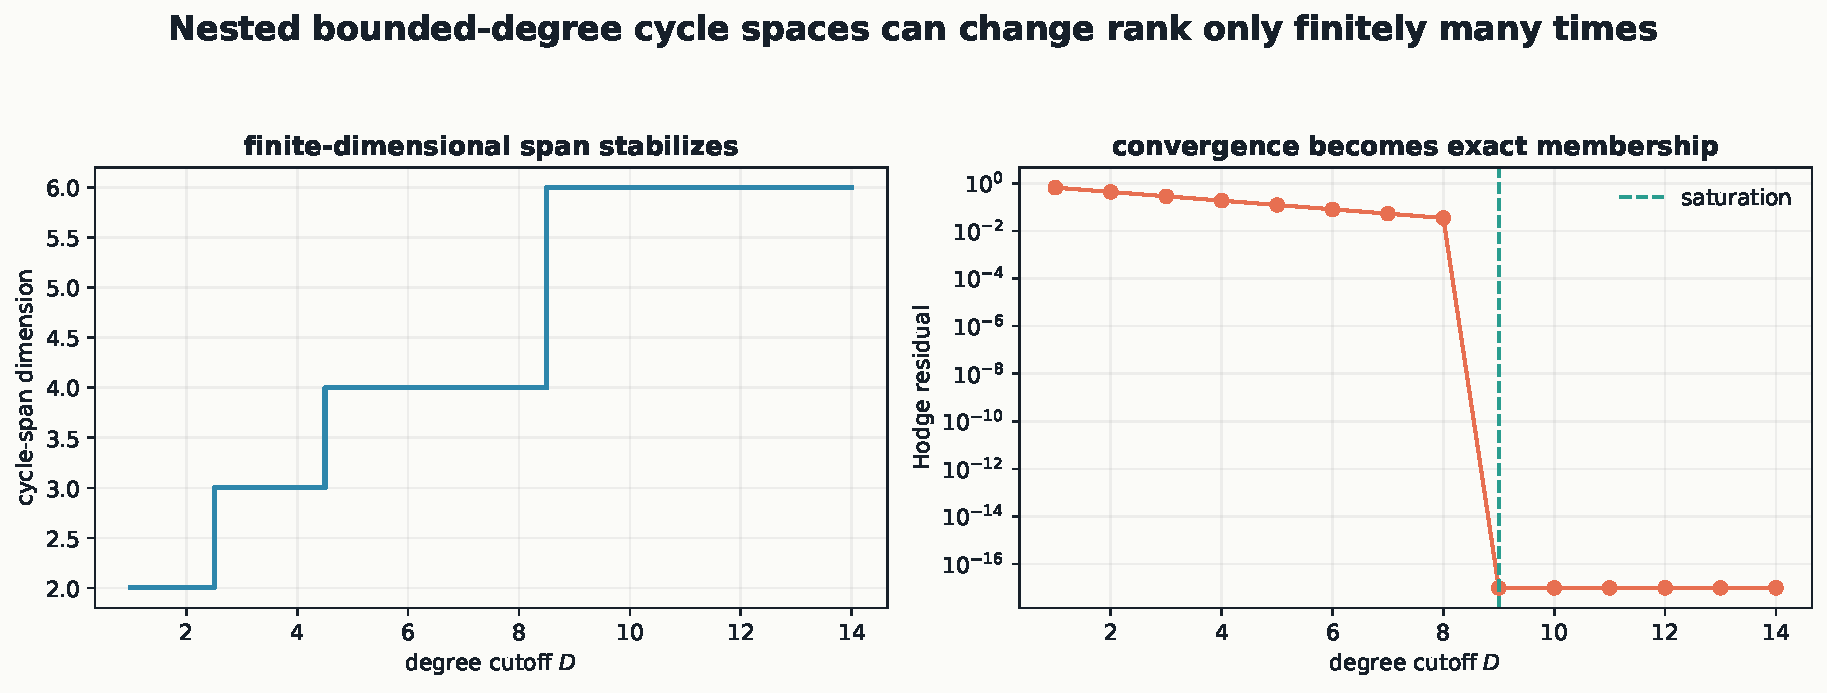
\includegraphics[width=0.9\textwidth]{12_finite_saturation.pdf}
\caption{The cycle span has a finite rank ceiling. Once the residual converges to zero, exact membership has already occurred at a finite stage.}
\end{figure}

\begin{resultbox}[Finite completion certificate]
If $H$ is a rational basis matrix of $\Hdg^p(X)$ and $C_D$ is the cycle matrix, then the Hodge conjecture for $(X,p)$ is equivalent to the existence of $D$ with
\[
\rank_{\Q} C_D=\rank_{\Q}[C_D\ H].
\]
Equivalently, the Hodge-restricted positive frame has positive minimum eigenvalue.
\end{resultbox}

\addcontentsline{toc}{part}{Part III. Support packets and correspondence reconstruction}

\chapter{Support verification and multiplicity recovery}
Let $Z\subseteq X$ be a closed algebraic subset and $j:X\setminus Z\hookrightarrow X$. The support exact sequence contains
\[
H_Z^{2p}(X,\Q)\longrightarrow H^{2p}(X,\Q)\xrightarrow{j^*}H^{2p}(X\setminus Z,\Q).
\]

\begin{theorem}[Exact support test]
A class $\alpha\in H^{2p}(X,\Q)$ is supported on $Z$ if and only if $j^*\alpha=0$.
\end{theorem}
\begin{proof}
This is exactness at the middle term.
\end{proof}

\begin{figure}[htbp]
\centering
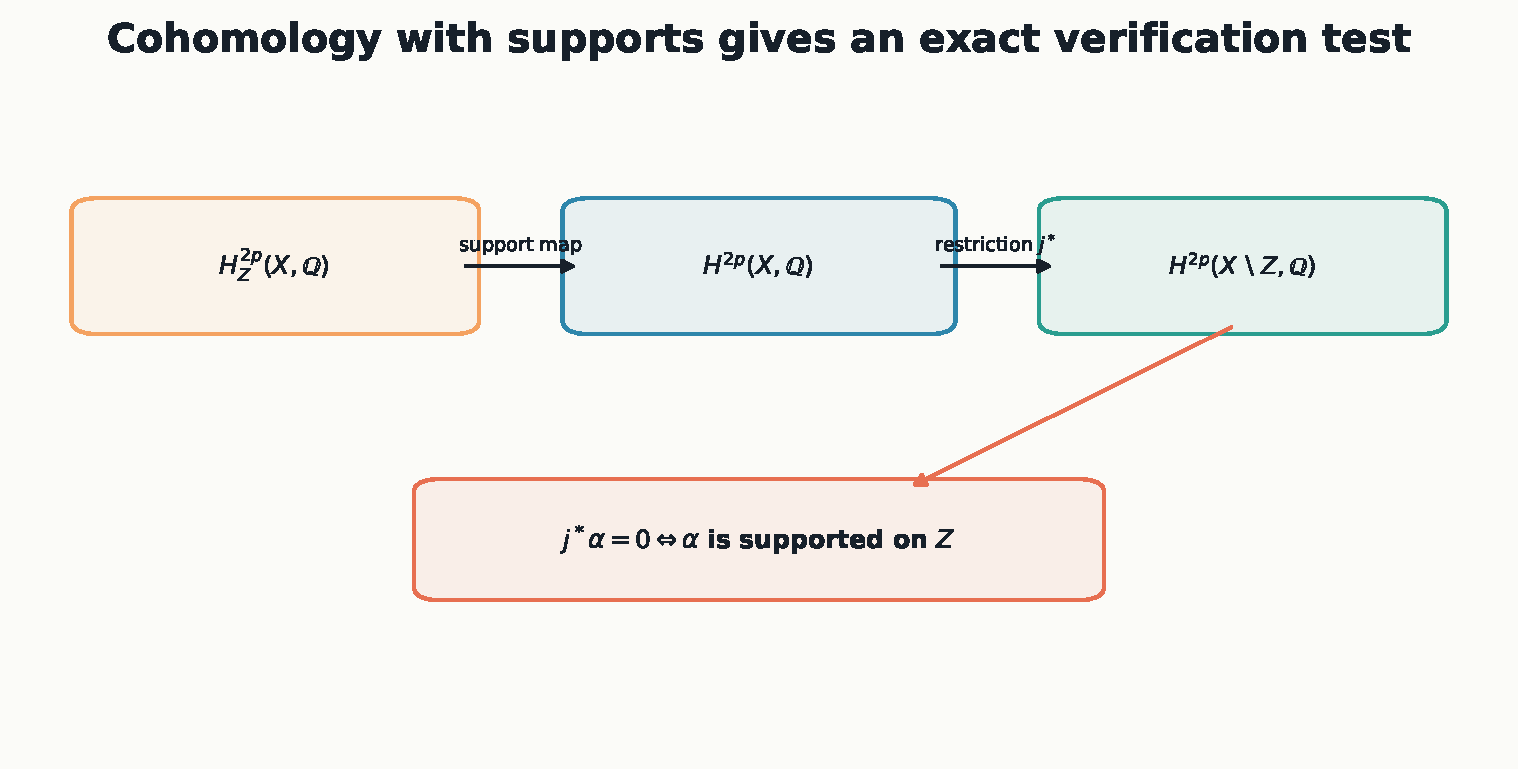
\includegraphics[width=0.82\textwidth]{14_support_exact_sequence.pdf}
\caption{Restriction to the complement provides an exact verification test for a proposed algebraic support.}
\end{figure}

Suppose the codimension-$p$ components are $Z_1,\ldots,Z_r$. Purity gives
\[
\alpha=\sum_{i=1}^r q_i[Z_i].
\]
Choose complementary test classes $\gamma_k$ and define
\[
M_{ki}=\int_X[Z_i]\smile\gamma_k,
\qquad
b_k=\int_X\alpha\smile\gamma_k.
\]
Then $Mq=b$. Removing dependent columns yields exact rational multiplicities.

\begin{figure}[htbp]
\centering
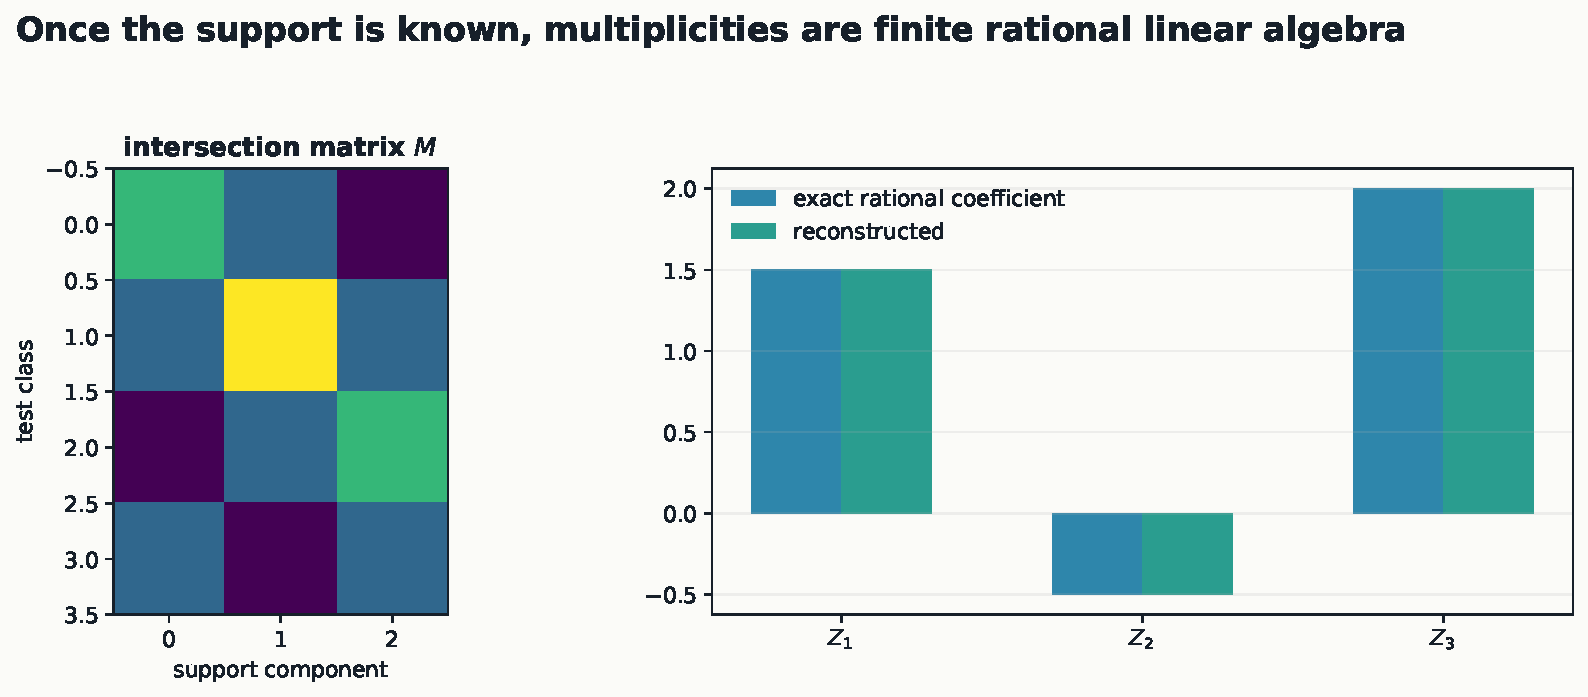
\includegraphics[width=0.9\textwidth]{13_support_multiplicity_reconstruction.pdf}
\caption{Once a support is verified, the cycle multiplicities are reconstructed by a finite rational linear system.}
\end{figure}

\chapter{Divisor-lowering correspondence channels}
\section{Degree bookkeeping}
Let $X$ have complex dimension $n$, let $V\subseteq H_{\mathrm{prim}}^{2p}(X,\Q)$ be a rational Hodge substructure, and let $Y_r$ be smooth projective. Choose correspondences
\[
\Gamma_r\in\CH^{n-p+1}(X\times Y_r)_{\Q},
\qquad
\Lambda_r\in\CH^{\dim Y_r+p-1}(Y_r\times X)_{\Q}.
\]
They induce
\[
A_r=(\Gamma_r)_*:V\to H^2(Y_r,\Q),
\qquad
B_r=(\Lambda_r)_*:H^2(Y_r,\Q)\to H^{2p}(X,\Q).
\]
Algebraic correspondences preserve rationality and shift Hodge type by the required bidegree.

\begin{theorem}[Invertible divisor-lowering transfer]
Suppose
\[
T=\sum_{r=1}^M B_rA_r
\]
preserves $V$ and is invertible on $V$. Then every rational Hodge class in $V$ is algebraic.
\end{theorem}
\begin{proof}
Let $\alpha\in V$ be of type $(p,p)$. Each $A_r\alpha$ is rational of type $(1,1)$ on $Y_r$, hence is the class of a rational divisor $D_r$ by the Lefschetz $(1,1)$ theorem. Therefore
\[
T\alpha=\sum_r(\Lambda_r)_*[D_r]
\]
is algebraic on $X$.

Let $\chi_T(t)=t^d+c_{d-1}t^{d-1}+\cdots+c_0$ be the characteristic polynomial on $V$. Invertibility means $c_0\ne0$. Cayley-Hamilton gives
\[
T^{-1}=-\frac{1}{c_0}\bigl(T^{d-1}+c_{d-1}T^{d-2}+\cdots+c_1I\bigr).
\]
Each power of $T$ is induced by compositions and rational sums of algebraic correspondences. Thus $T^{-1}$ preserves algebraic cycle classes. Hence $\alpha=T^{-1}(T\alpha)$ is algebraic.
\end{proof}

\begin{figure}[htbp]
\centering
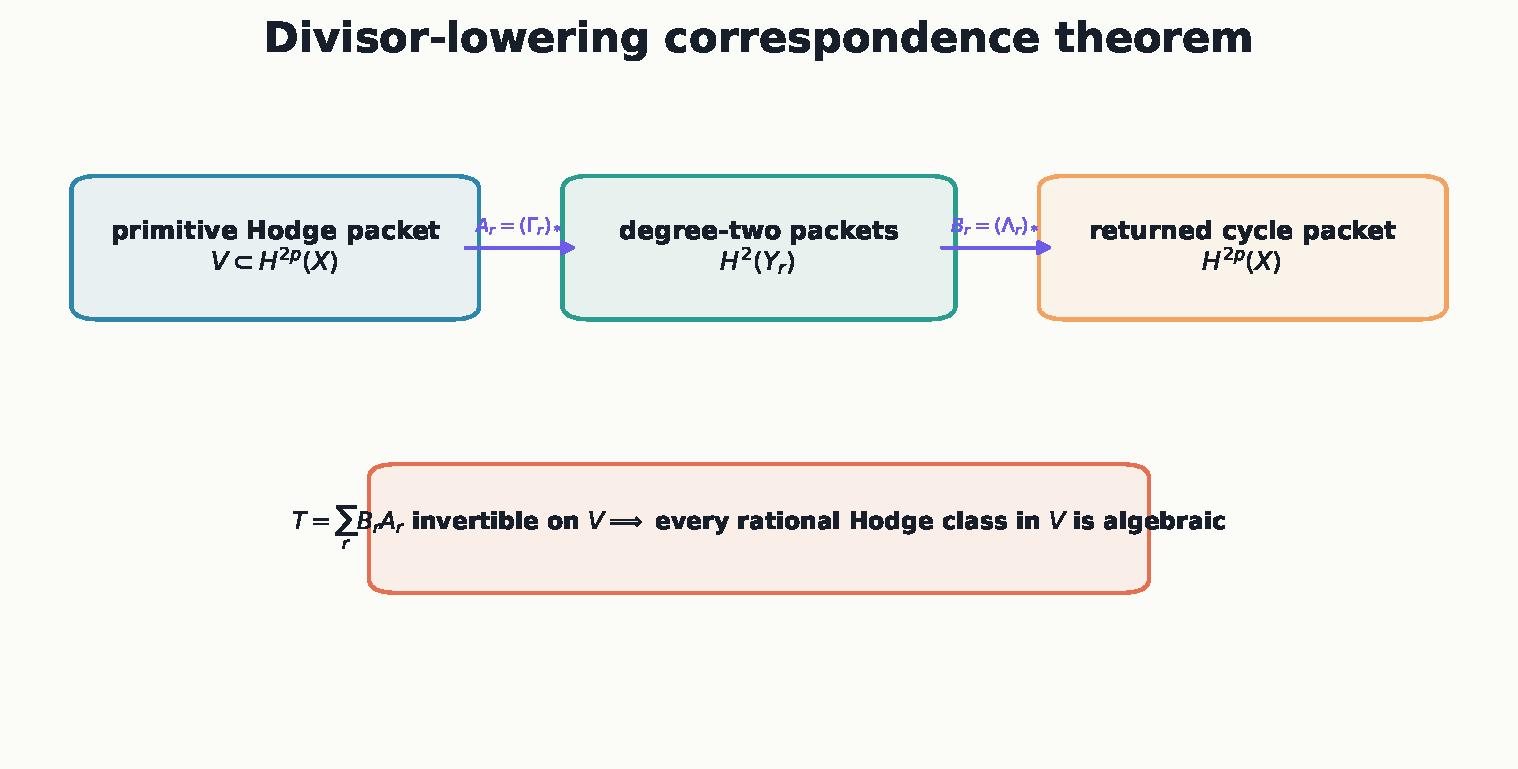
\includegraphics[width=0.86\textwidth]{15_divisor_lowering_transfer.pdf}
\caption{A primitive Hodge class is lowered to divisor degree, algebraized there, and returned through an invertible transfer.}
\end{figure}

\begin{figure}[htbp]
\centering
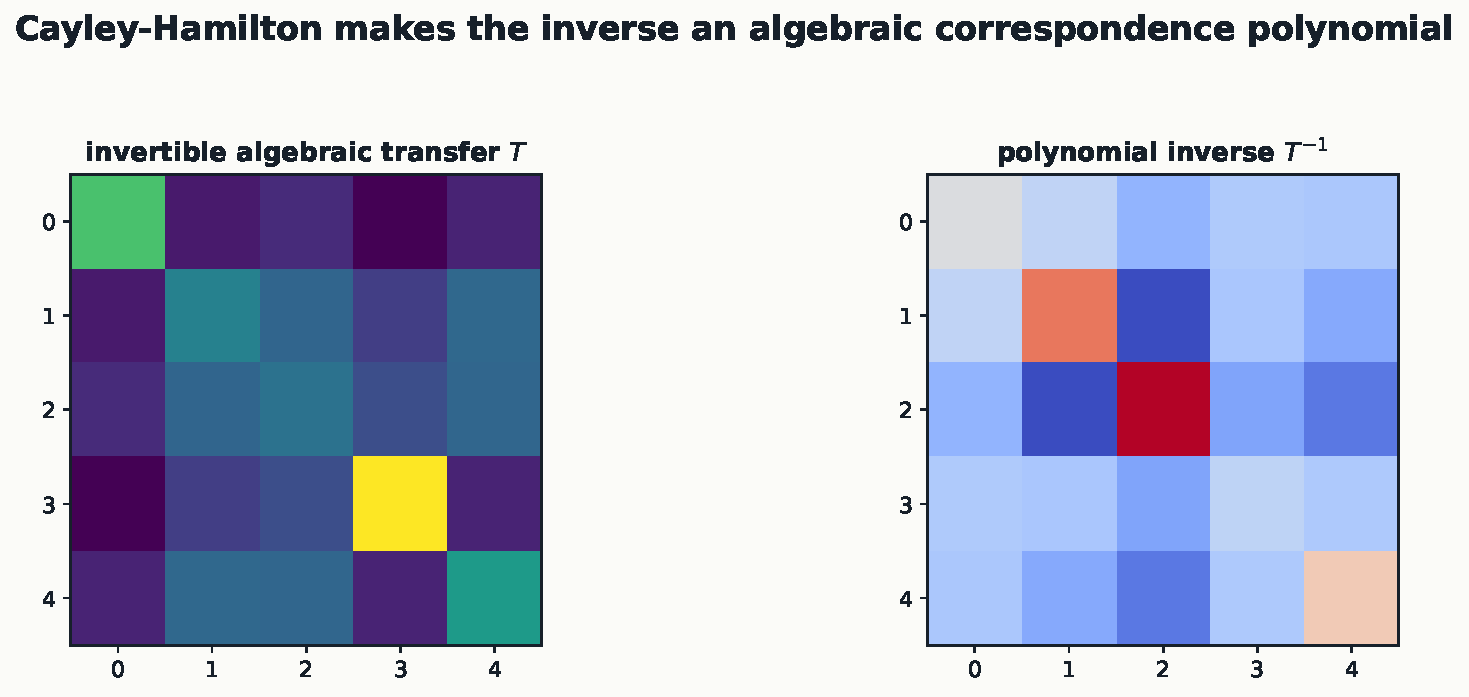
\includegraphics[width=0.82\textwidth]{18_cayley_hamilton_inverse.pdf}
\caption{The inverse transfer is a rational polynomial in the original algebraic correspondence operator.}
\end{figure}

\section{Positive multi-channel form}
Assume the polarized adjoint $A_r^\dagger$ is realized by an algebraic return correspondence $B_r$. This is an additional geometric hypothesis, not an automatic consequence in arbitrary settings. Then
\[
T=\sum_rA_r^\dagger A_r
\]
is positive and
\[
\langle v,Tv\rangle=\sum_r\|A_rv\|^2.
\]
Therefore
\[
\ker T=\bigcap_r\ker A_r.
\]
Joint injectivity of the lowering channels is enough.

\begin{figure}[htbp]
\centering
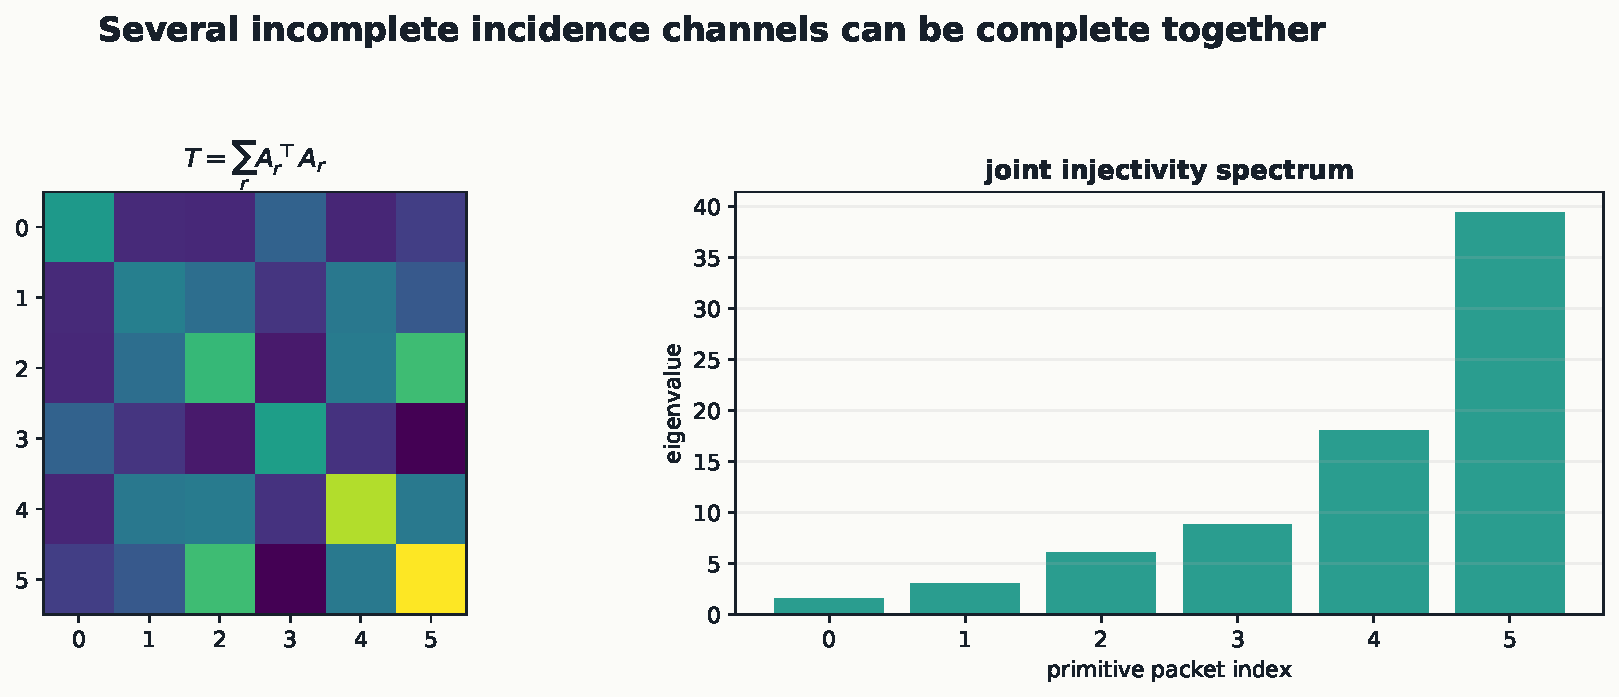
\includegraphics[width=0.88\textwidth]{16_positive_correspondence_frame.pdf}
\caption{Several incidence channels may be individually incomplete while their positive sum is invertible.}
\end{figure}

\begin{figure}[htbp]
\centering
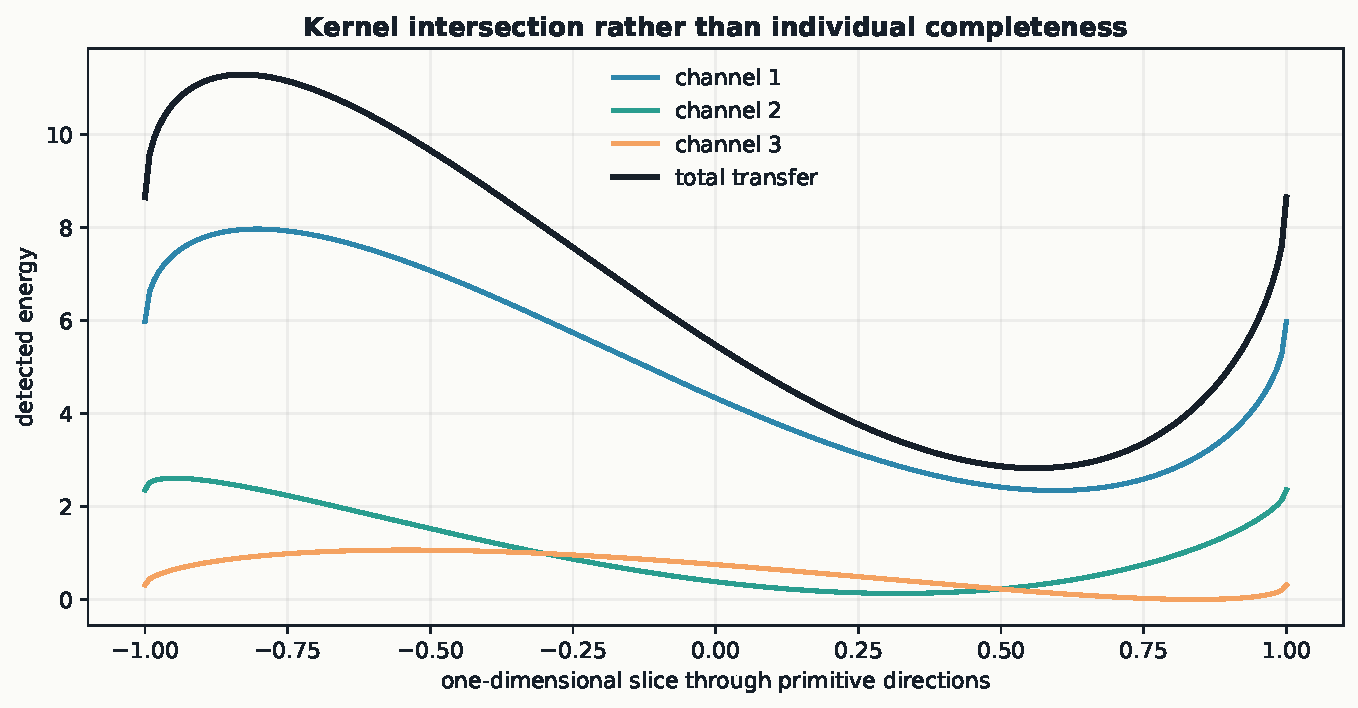
\includegraphics[width=0.82\textwidth]{17_multi_incidence_kernel_intersection.pdf}
\caption{The correct criterion is the vanishing of the joint kernel, not completeness of one channel.}
\end{figure}

\begin{corollary}[Finite Gram certificate]
Choose a rational basis $e_1,\ldots,e_d$ of $V$. If
\[
G_{ij}=\sum_r\langle A_re_i,A_re_j\rangle_{Y_r}
\]
has nonzero determinant, every rational Hodge class in $V$ is algebraic.
\end{corollary}

\chapter{Family propagation}
Let $\pi:\mathcal X\to S$ and $\rho_r:\mathcal Y_r\to S$ be smooth projective families over a connected base. Relative algebraic correspondences induce morphisms of Gauss-Manin local systems. In a flat rational trivialization, their transfer matrix is constant.

\begin{theorem}[Propagation of invertibility]
If a relative transfer $T_s$ is invertible on one fiber $s_0$, it is invertible on every fiber in the connected base on which the local systems and correspondences are defined.
\end{theorem}
\begin{proof}
The determinant of the constant rational matrix representing the local-system morphism is locally constant. It is nonzero at $s_0$, hence everywhere on the connected base.
\end{proof}

\begin{figure}[htbp]
\centering
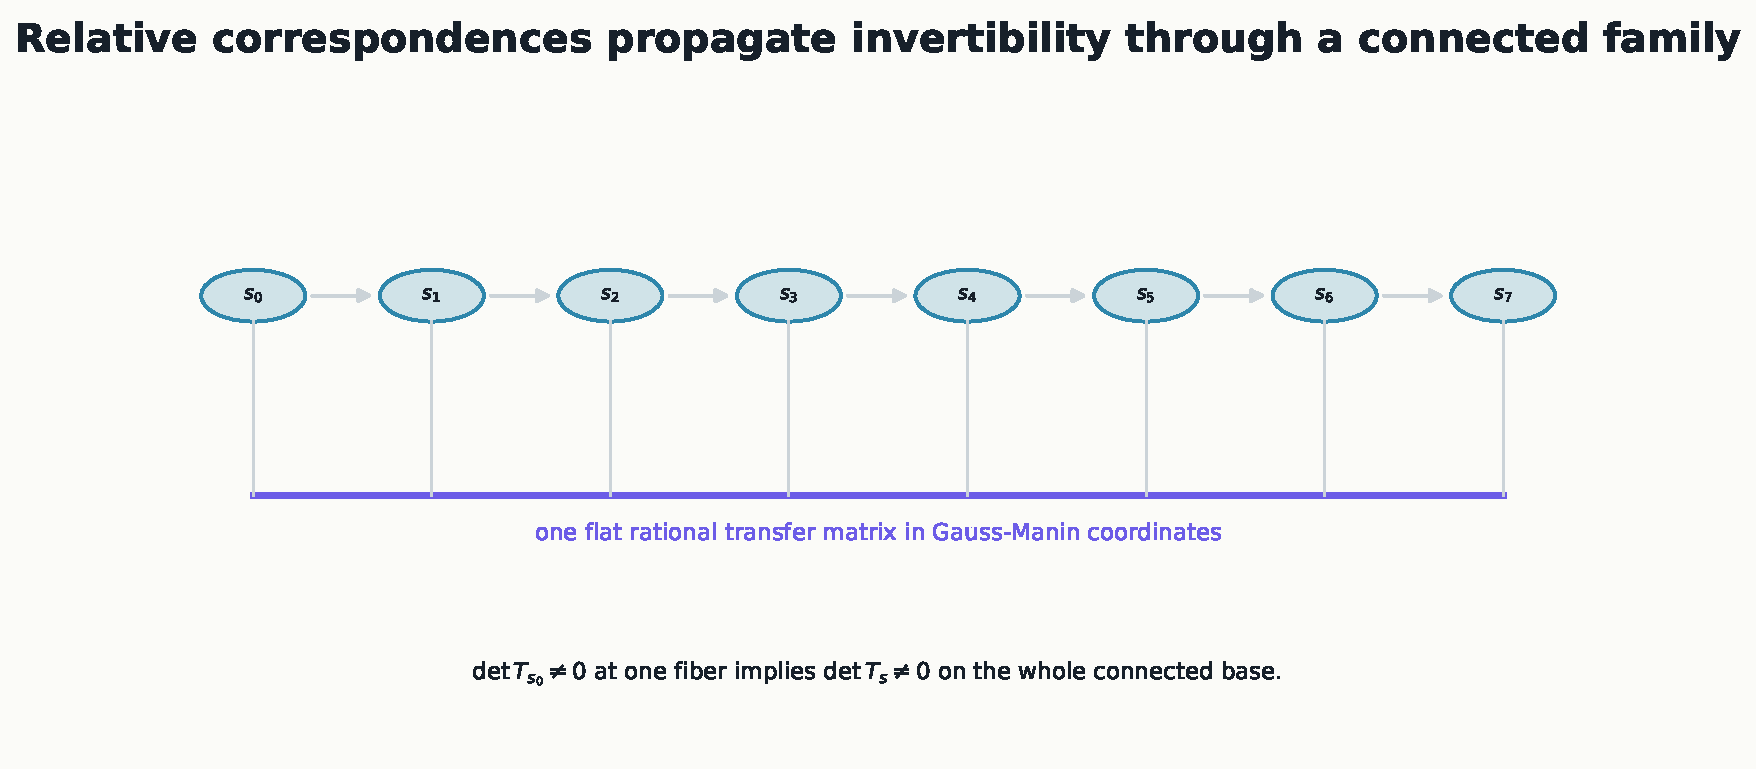
\includegraphics[width=0.83\textwidth]{19_family_propagation.pdf}
\caption{One verified fiber can control a connected smooth family when the correspondence is relative and flat.}
\end{figure}

\addcontentsline{toc}{part}{Part IV. Closed branches and classical validation cases}

\chapter{Geometric closure rules}
\section{Affine pavings}
\begin{theorem}[Affine-paving branch]
If $X$ admits a finite filtration whose successive differences are affine spaces, then the cycle class map
\[
\CH^p(X)_{\Q}\to H^{2p}(X,\Q)
\]
is surjective for every $p$.
\end{theorem}
\begin{proof}[Proof sketch]
Induct through the filtration using localization for Chow groups and cohomology. Each affine cell contributes one even-degree generator represented by the closure of that cell. No odd cohomology is introduced.
\end{proof}

\section{Projective bundles, blow-ups, and descent}
\begin{proposition}[Projective-bundle closure]
If the rational Hodge conjecture holds for $X$, it holds for $\mathbb P(E)\to X$.
\end{proposition}
\begin{proof}
The projective-bundle formula expresses cohomology as a direct sum of powers of the algebraic hyperplane class times pullbacks of cohomology from $X$.
\end{proof}

\begin{proposition}[Blow-up closure]
If it holds for $X$ and a smooth center $Z$, it holds for $\operatorname{Bl}_ZX$.
\end{proposition}
\begin{proof}
Use the standard blow-up cohomology decomposition. The new summands are Tate twists of cohomology from $Z$ multiplied by powers of the algebraic exceptional divisor.
\end{proof}

\begin{proposition}[Generically finite descent]
Let $f:Y\to X$ be proper and generically finite of degree $d$ between smooth projective varieties of equal dimension. If the conjecture holds for $Y$, it holds for $X$.
\end{proposition}
\begin{proof}
For a Hodge class $\alpha$ on $X$, the pullback $f^*\alpha$ is algebraic on $Y$. Push forward and use $f_*f^*\alpha=d\alpha$.
\end{proof}

\begin{figure}[htbp]
\centering
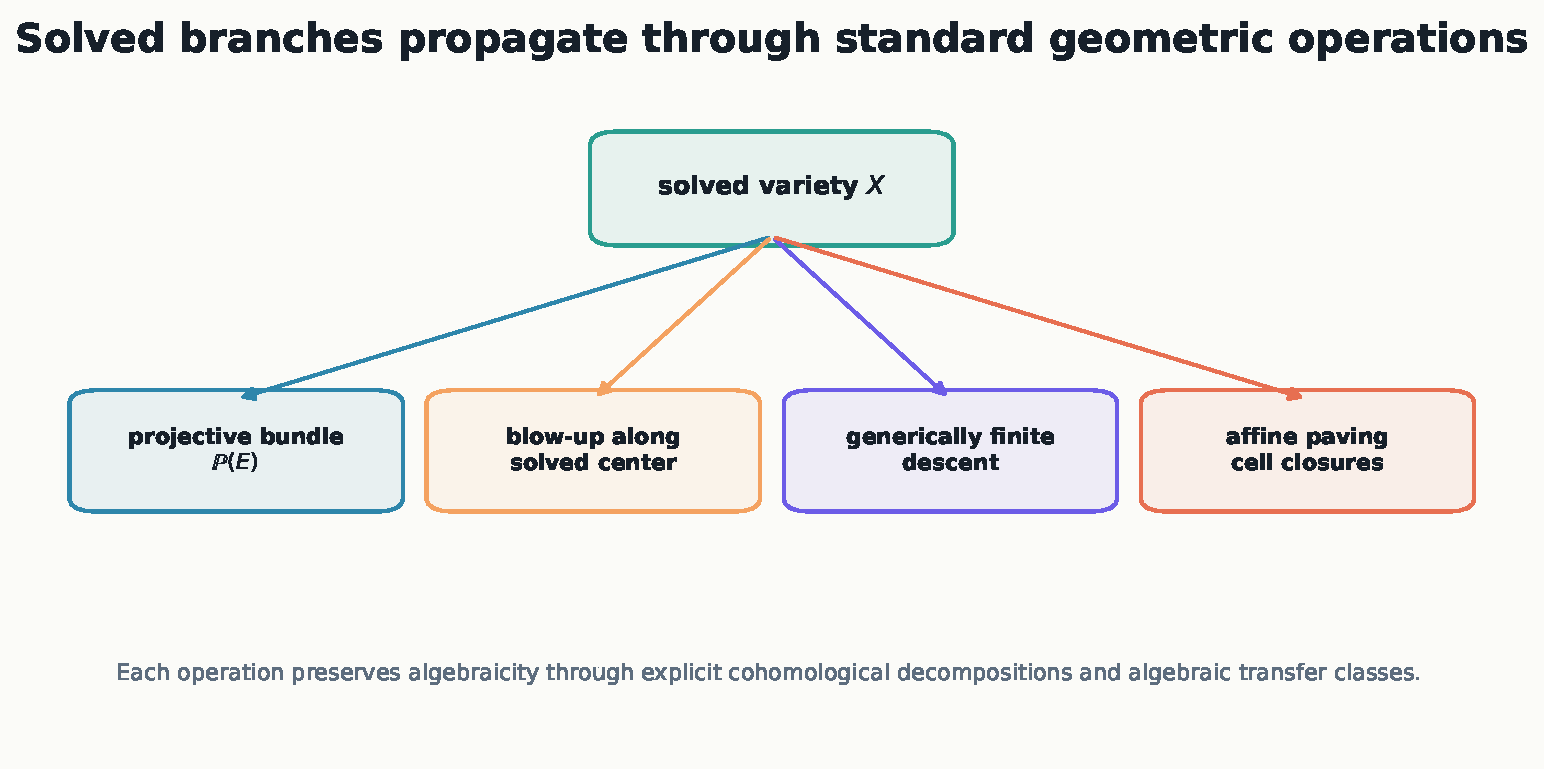
\includegraphics[width=0.84\textwidth]{20_geometric_closure_operations.pdf}
\caption{Solved branches propagate through several exact algebraic operations.}
\end{figure}

\chapter{Cubic fourfolds as a validation of the transfer theorem}
Let $X\subset\mathbb P^5$ be a smooth cubic fourfold and let $F(X)$ be its Fano variety of lines. The universal incidence variety
\[
P=\{(\ell,x):x\in\ell\}\subset F(X)\times X
\]
induces the Abel-Jacobi map
\[
A=p_*q^*:H^4_{\mathrm{prim}}(X,\Q)\to H^2_{\mathrm{prim}}(F(X),\Q).
\]
Beauville and Donagi proved that this is a polarized Hodge isomorphism up to the standard twist \cite{BeauvilleDonagi}. The polarized adjoint is represented by an algebraic incidence return after inserting the appropriate power of the Pluecker class. Therefore the divisor-lowering transfer is invertible.

\begin{resultbox}[Classical validation]
A primitive rational $(2,2)$ class on a cubic fourfold is sent to a rational $(1,1)$ class on $F(X)$, represented by a divisor. The algebraic return correspondence and its polynomial inverse reconstruct an algebraic codimension-two class on $X$. This is a validation of the packet criterion, not a claim of a new proof of the classical cubic-fourfold result.
\end{resultbox}

\begin{figure}[htbp]
\centering
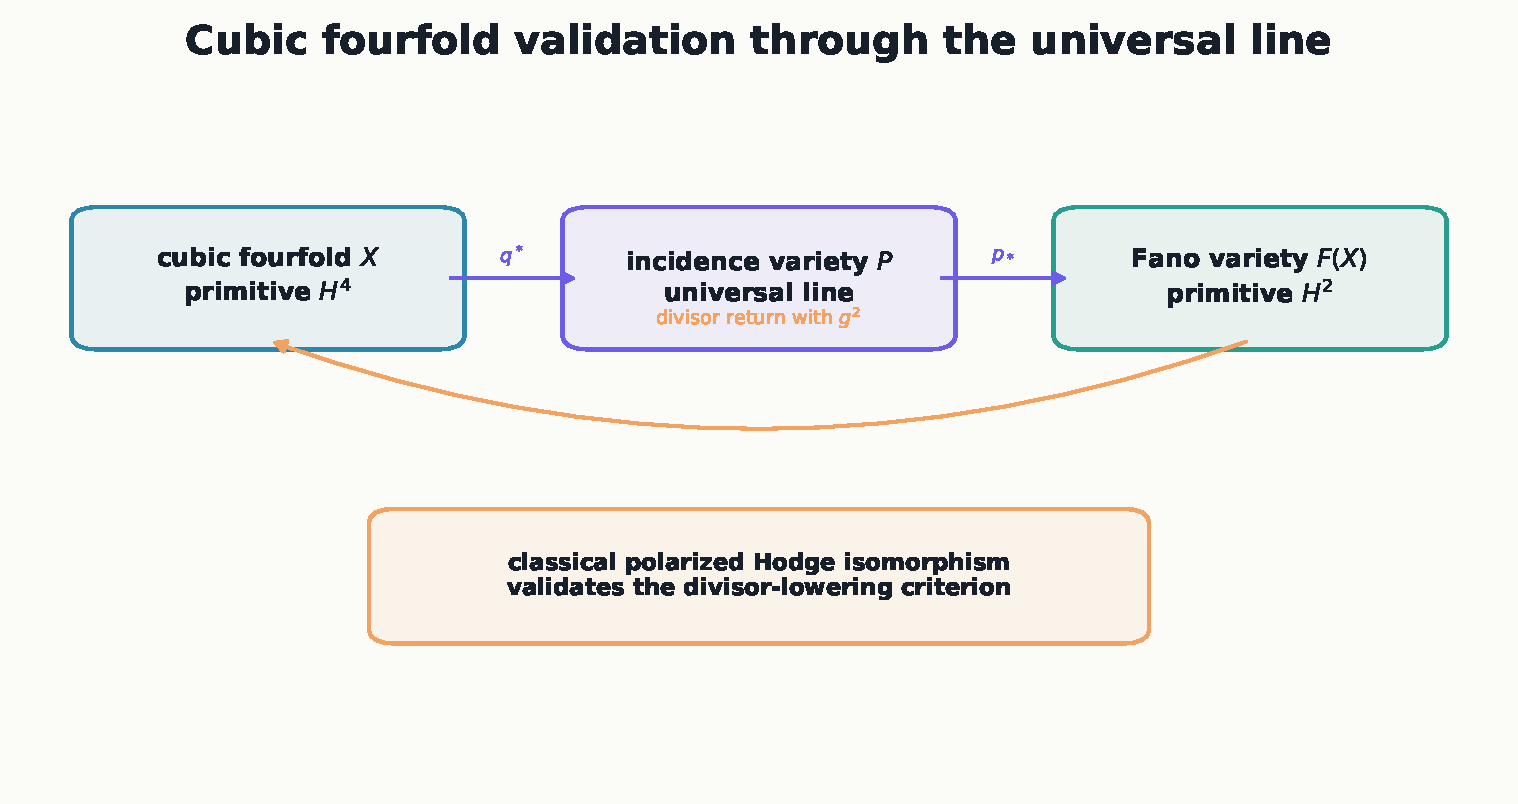
\includegraphics[width=0.86\textwidth]{21_cubic_fourfold_incidence.pdf}
\caption{The universal line lowers primitive degree-four cohomology to divisor degree on the Fano variety.}
\end{figure}

\begin{figure}[htbp]
\centering
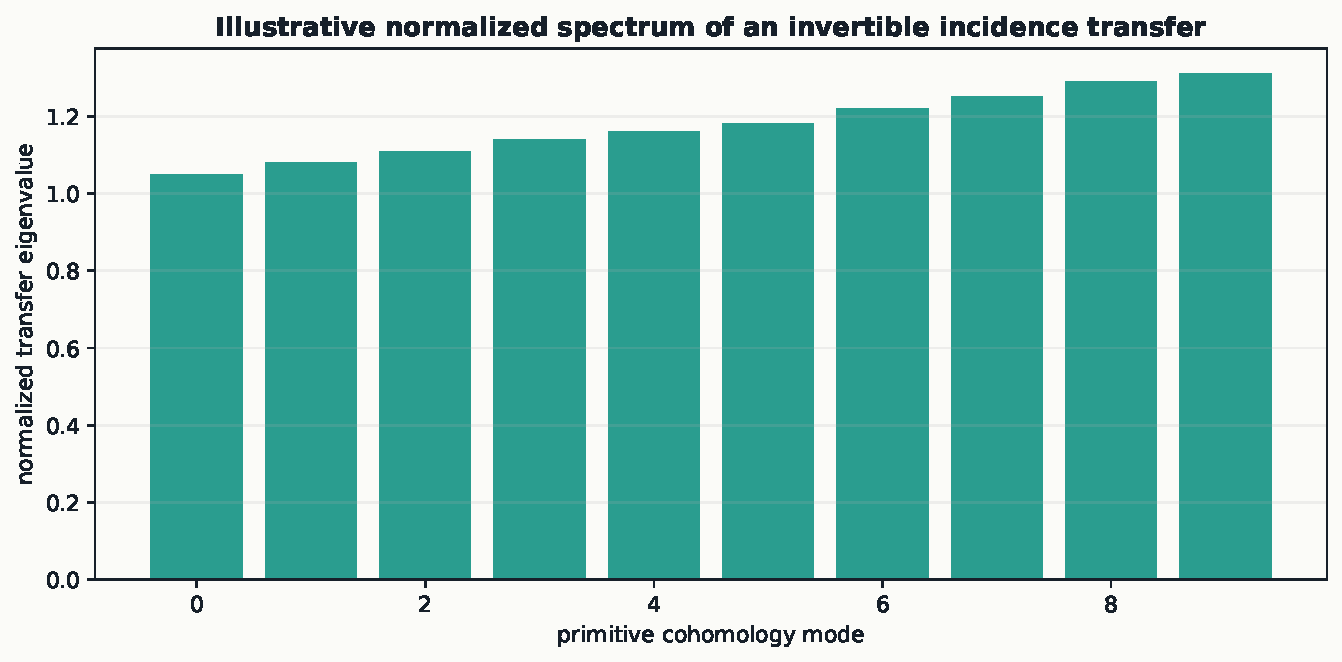
\includegraphics[width=0.72\textwidth]{22_cubic_transfer_spectrum.pdf}
\caption{Illustrative normalized transfer spectrum. The mathematical criterion is nonvanishing, not the displayed toy values.}
\end{figure}

\chapter{Gushel-Mukai validation channels}
Debarre and Kuznetsov construct line and plane incidence correspondences relating vanishing middle cohomology of suitable Gushel-Mukai varieties to primitive degree-two cohomology of associated double EPW sextics \cite{DebarreKuznetsov}. In the ranges where the polarized Hodge isomorphisms are established, the same divisor-lowering theorem applies.

\begin{itemize}
\item For suitable GM fourfolds, the vanishing $H^4$ packet is lowered by universal lines to divisor degree.
\item For suitable GM sixfolds, the vanishing $H^6$ packet is lowered by universal planes to divisor degree.
\item Ambient and tautological classes are treated separately and are algebraic.
\end{itemize}

\begin{figure}[htbp]
\centering
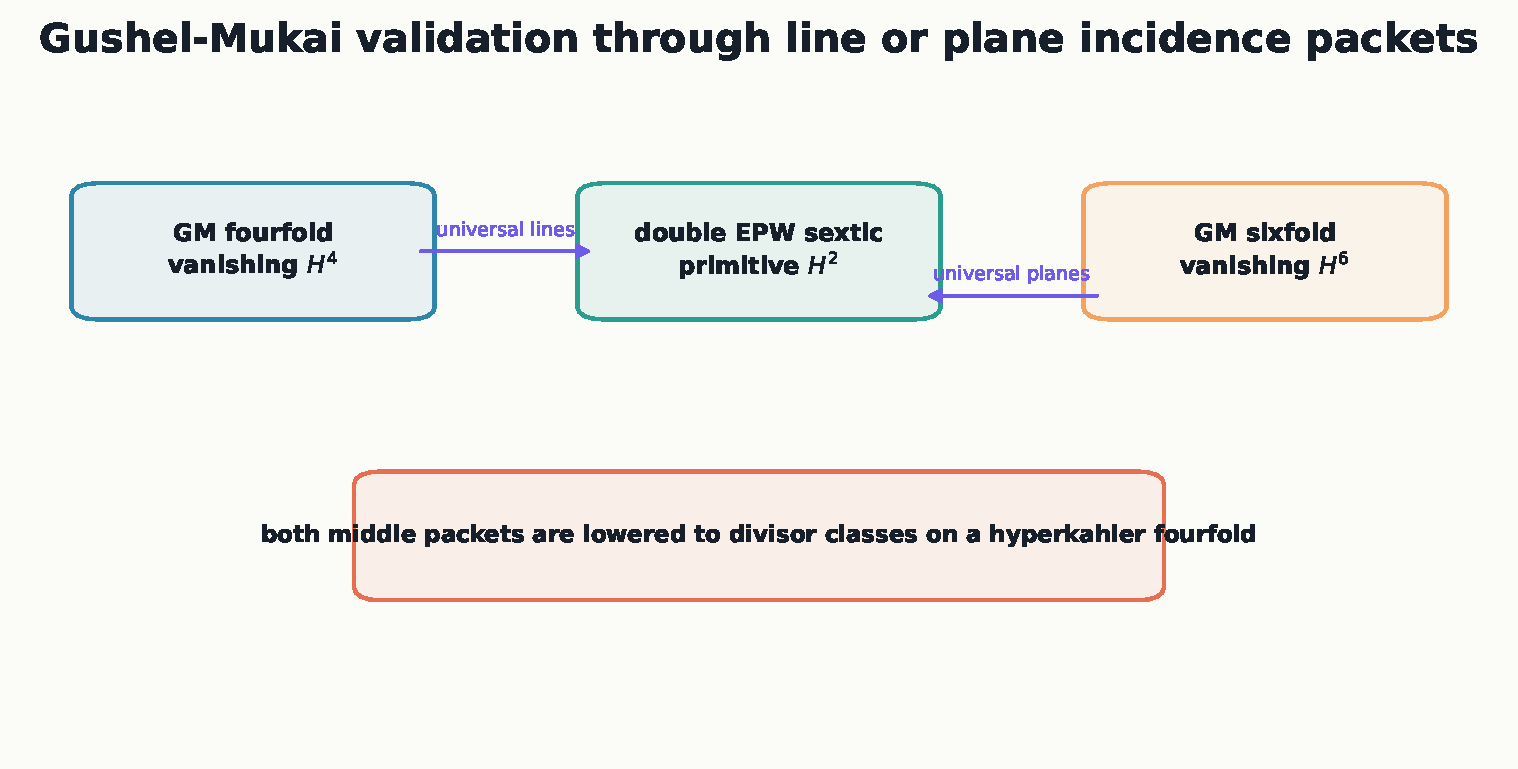
\includegraphics[width=0.84\textwidth]{23_gushel_mukai_correspondences.pdf}
\caption{Line and plane incidence packets lower middle cohomology to degree two on an associated hyperkaehler fourfold.}
\end{figure}

\addcontentsline{toc}{part}{Part V. The analytic and K-theoretic branch}

\chapter{Hodge packets in topological K-theory}
For finite CW complexes, the rational topological Chern character gives
\[
\operatorname{ch}_{\mathrm{top}}:K^0_{\mathrm{top}}(X)\otimes\Q\xrightarrow{\sim}H^{\mathrm{even}}(X,\Q).
\]
For smooth projective $X$, the algebraic Chern character identifies algebraic $K$-theory rationally with the Chow ring after the usual filtration. Thus the rational Hodge conjecture for all degrees is equivalent to algebraization of topological $K$-classes whose Chern-character components are rational Hodge classes \cite{AtiyahHirzebruch}.

\section{Adams degree projectors}
For integer $m\ge2$, Adams operations satisfy
\[
\operatorname{ch}_q(\psi^m\xi)=m^q\operatorname{ch}_q(\xi).
\]
Define
\[
e_p^{(m)}=\prod_{\substack{0\le q\le\dim X\\q\ne p}}
\frac{\psi^m-m^qI}{m^p-m^q}.
\]
Then
\[
\operatorname{ch}_q(e_p^{(m)}\xi)=\delta_{pq}\operatorname{ch}_p(\xi).
\]
This exactly isolates codimension $p$ inside a topological $K$-packet.

\begin{figure}[htbp]
\centering
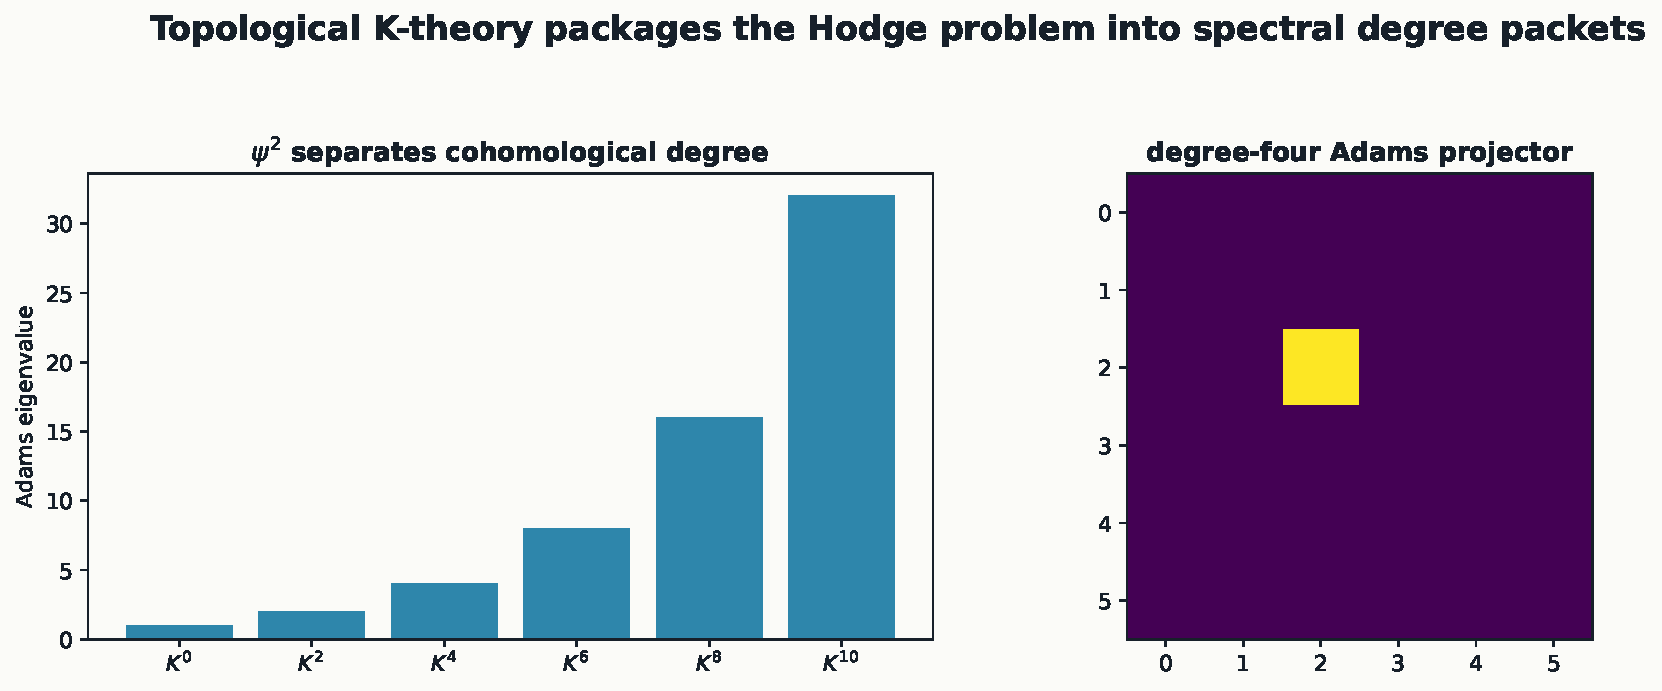
\includegraphics[width=0.86\textwidth]{24_adams_degree_projector.pdf}
\caption{Adams eigenvalues separate cohomological degrees and yield an exact spectral projector onto degree four in the toy model.}
\end{figure}

\chapter{Nonlinear Dolbeault obstruction packets}
Let $E$ be a smooth complex bundle and consider a candidate $(0,1)$-connection. After gauge fixing, write the integrability equation abstractly as
\[
F(a)=f+La+B(a,a)=0,
\]
where $L$ is the linearized operator and $B$ is a bounded bilinear term. Assume a Fredholm splitting of the target
\[
I=Q+\Pi,
\]
where $Q$ projects onto the range of $L$ and $\Pi$ onto a finite-dimensional obstruction space. Let $R$ be a right inverse of $L$ on the range.

\begin{theorem}[Range-packet contraction]
Assume
\[
\|R\|\le M,
\qquad
\|B(a,b)\|\le C\|a\|\|b\|,
\qquad
4CM^2\|Qf\|<1.
\]
Then the map
\[
\mathcal T(a)=-RQ(f+B(a,a))
\]
has a unique fixed point in the ball $\|a\|\le2M\|Qf\|$. At the fixed point, the range component of $F(a)$ vanishes. The remaining obstruction is
\[
\Phi=\Pi(f+B(a,a)).
\]
The full integrability equation holds if and only if $\Phi=0$.
\end{theorem}
\begin{proof}
For $\|a\|\le r=2M\|Qf\|$,
\[
\|\mathcal T(a)\|\le M\|Qf\|+MC r^2\le r
\]
under the stated bound. Moreover
\[
\|\mathcal T(a)-\mathcal T(b)\|
\le MC(\|a\|+\|b\|)\|a-b\|<\|a-b\|.
\]
Banach's fixed-point theorem gives the solution. Applying $Q$ to the equation proves range cancellation. The remaining component is precisely $\Phi$.
\end{proof}

\begin{figure}[htbp]
\centering
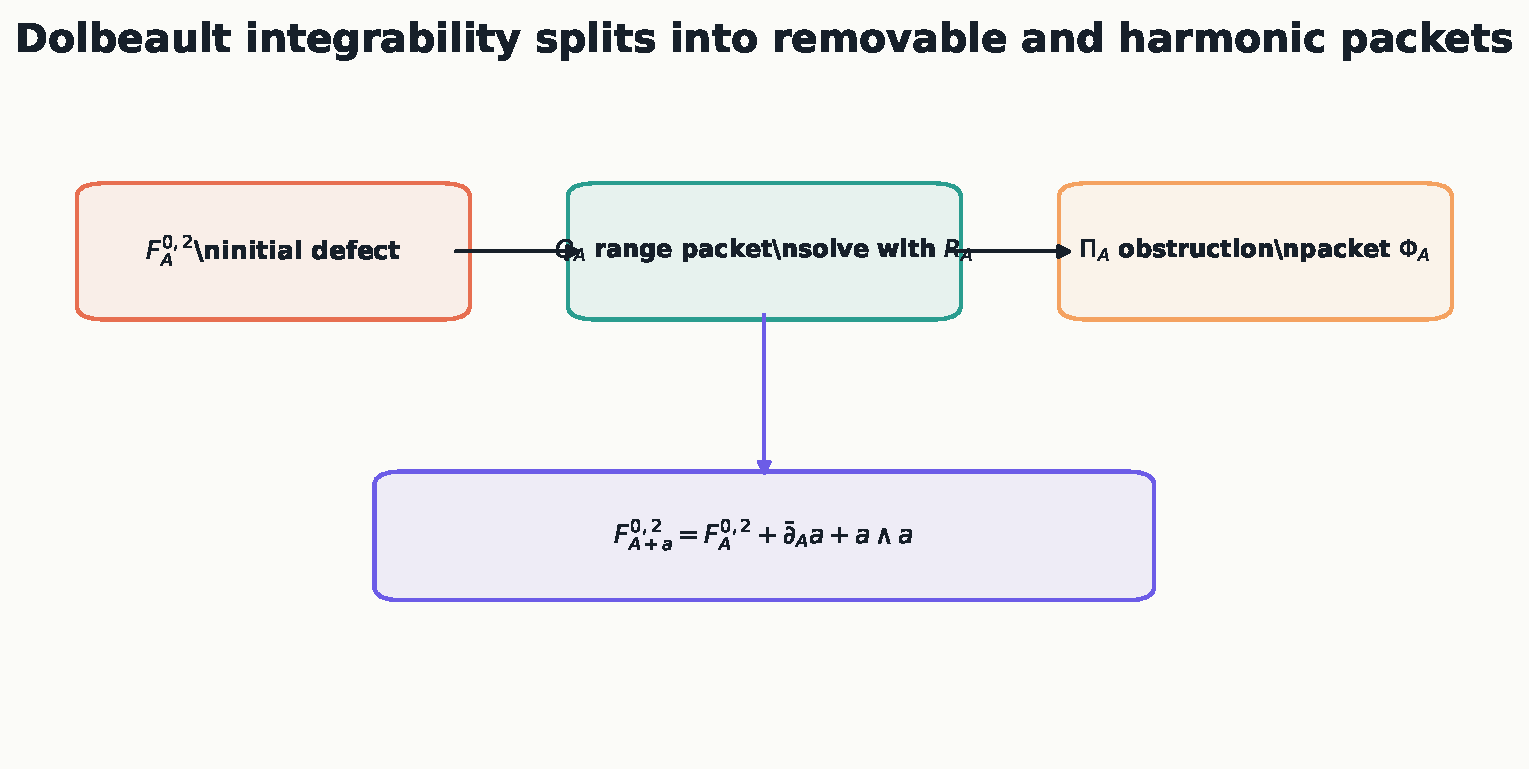
\includegraphics[width=0.84\textwidth]{25_dolbeault_obstruction_split.pdf}
\caption{The nonlinear equation splits into a removable range packet and a finite effective obstruction packet.}
\end{figure}

\begin{figure}[htbp]
\centering
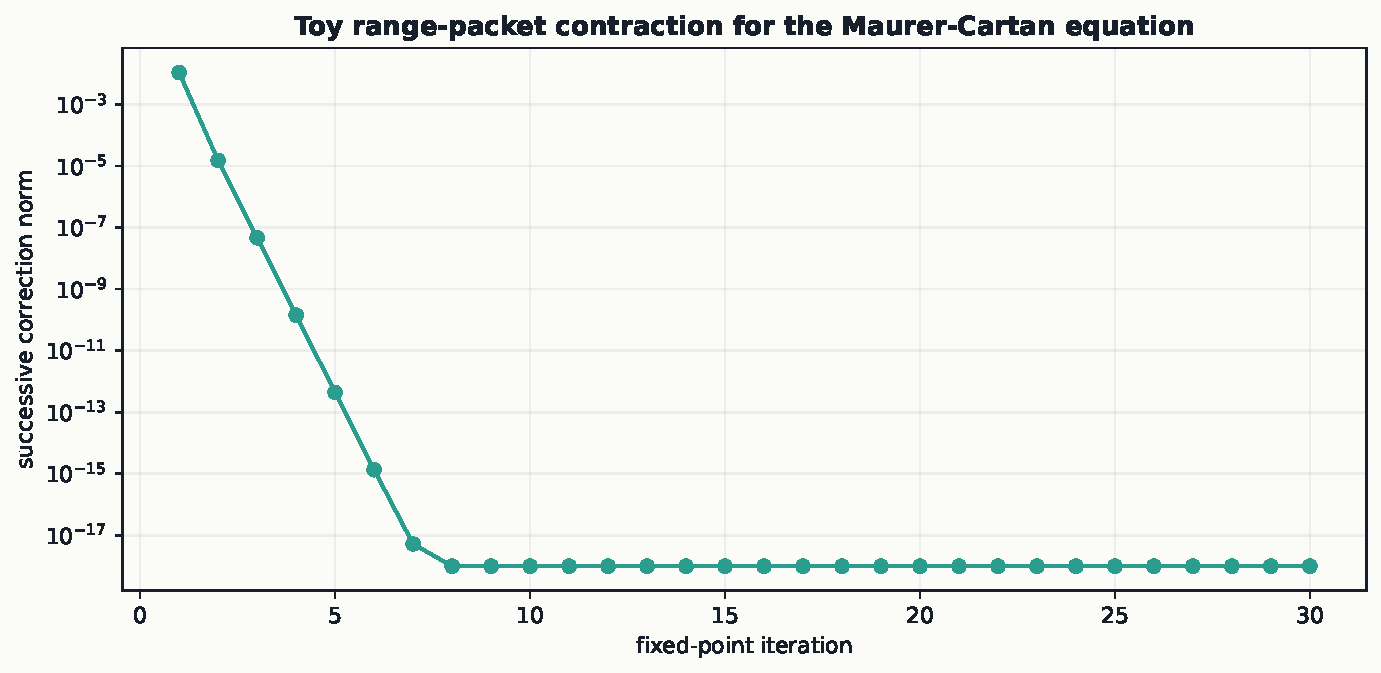
\includegraphics[width=0.72\textwidth]{26_dolbeault_contraction.pdf}
\caption{Reproducible finite model of geometric contraction in the removable packet.}
\end{figure}

\section{A positive spectral microscope}
Large ample twists can make integrability defects visible in the asymptotic degree distribution of Dolbeault-Dirac kernels. Charbonneau and Stern obtain asymptotic Hodge filtrations in which positive coefficients depend on powers of $F_A^{0,2}$ \cite{CharbonneauStern}. Schematically,
\[
\Tr(P_{2j}\Pi_{A,k})
=c_{n,j}k^{n-2j}\|(F_A^{0,2})^{\wedge j}\|_{L^2}^2+O(k^{n-2j-1}),
\qquad c_{n,j}>0.
\]
This detects nonintegrability. It does not by itself remove the defect.

\begin{figure}[htbp]
\centering
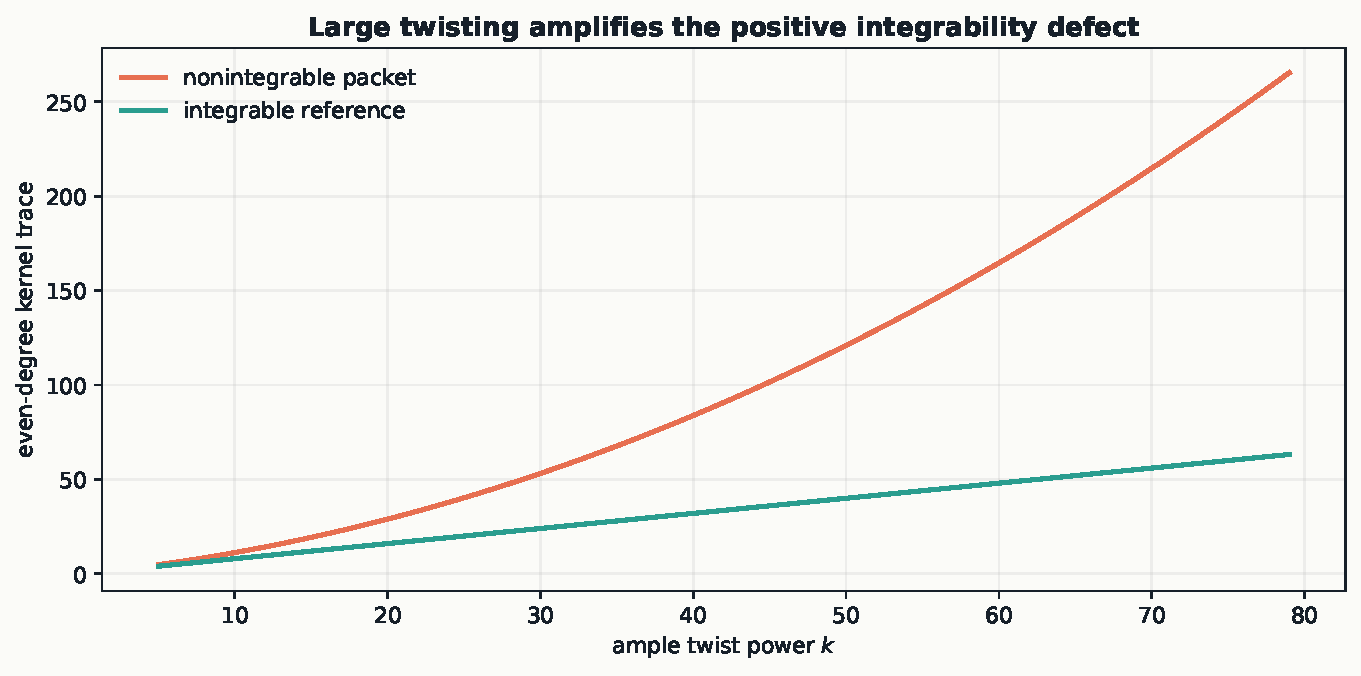
\includegraphics[width=0.74\textwidth]{27_asymptotic_integrability_packet.pdf}
\caption{Ample twisting acts as a spectral microscope for a positive integrability defect.}
\end{figure}

\section{Trace blindness and the true missing bridge}
Chern characters control traces of powers of curvature. An endomorphism-valued obstruction can be nonzero while all such trace moments vanish. A nilpotent block gives the elementary counterexample.

\begin{figure}[htbp]
\centering
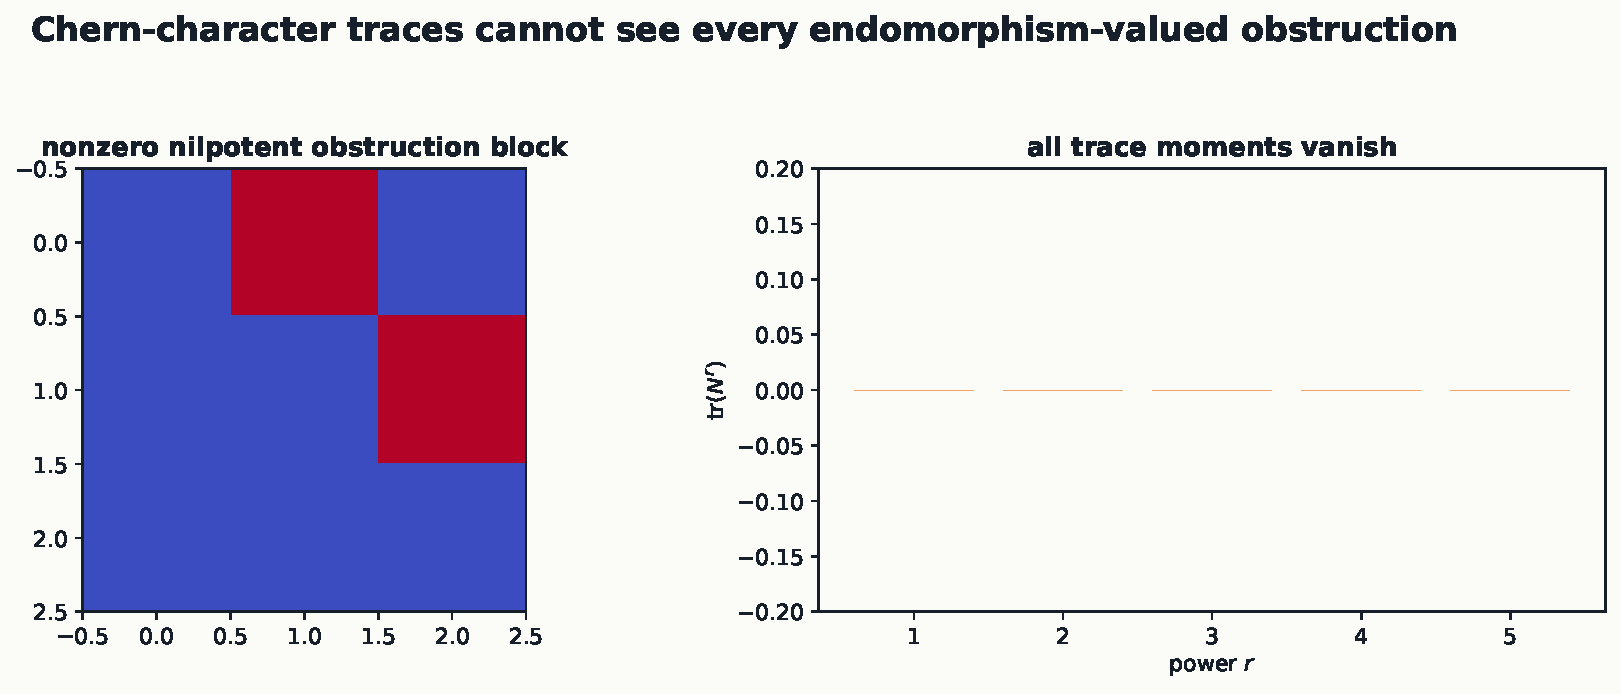
\includegraphics[width=0.8\textwidth]{28_trace_blindness.pdf}
\caption{A nonzero nilpotent obstruction can be invisible to every trace power. Hodge-type Chern data do not automatically kill the full matrix obstruction.}
\end{figure}

\begin{openproblem}[Analytic bridge]
The unresolved analytic theorem is not the range equation. It is a positive saturation statement forcing the finite obstruction packet $\Phi$ to vanish for every rational Hodge $K$-packet after allowable stabilization. Proving that statement in general would be essentially a K-theoretic form of the Hodge conjecture.
\end{openproblem}

\section{Consequences of the obstruction split}
The obstruction split prevents a common logical error. Solving the projected range equation does not solve the original integrability problem unless the complementary packet also vanishes. The calculus therefore records three distinct outcomes. First, if $\Pi=0$, the problem is unobstructed and the contraction theorem gives an actual integrable structure. Second, if $\Pi\ne0$ but $\Phi=0$ for geometric reasons, the correction again closes. Third, if $\Phi\ne0$, the method has produced a finite certificate explaining exactly why that representative cannot be algebraized by the chosen deformation.

This creates a practical research program. One can refine the finite obstruction space by symmetry, monodromy, support, or arithmetic phase, obtaining
\[
\Phi=\sum_{\lambda}\Phi_{\lambda}.
\]
Since the decomposition is complete, integrability is equivalent to the simultaneous vanishing of all children. Different geometric arguments may eliminate different children. A symmetry packet may vanish by representation theory, a support packet by localization, and an arithmetic packet by compatibility across reductions. The analytic branch therefore remains useful even before the general bridge is proved: it supplies exact special-case theorems whenever all obstruction children can be eliminated.

The negative controls are equally important. Ample twisting can amplify $F_A^{0,2}$ in a spectral observable without reducing it. Direct-sum stabilization adds positive defect energies for block-diagonal connections. Trace identities may miss nilpotent components. These facts rule out several tempting but invalid shortcuts and keep the remaining theorem sharply stated.


\addcontentsline{toc}{part}{Part VI. Atomic status ledger and focused next theorem}

\chapter{Dependency graph and proof status}
The project separates proved statements, classical inputs, conditional mechanisms, and open bridges.

\begin{figure}[htbp]
\centering
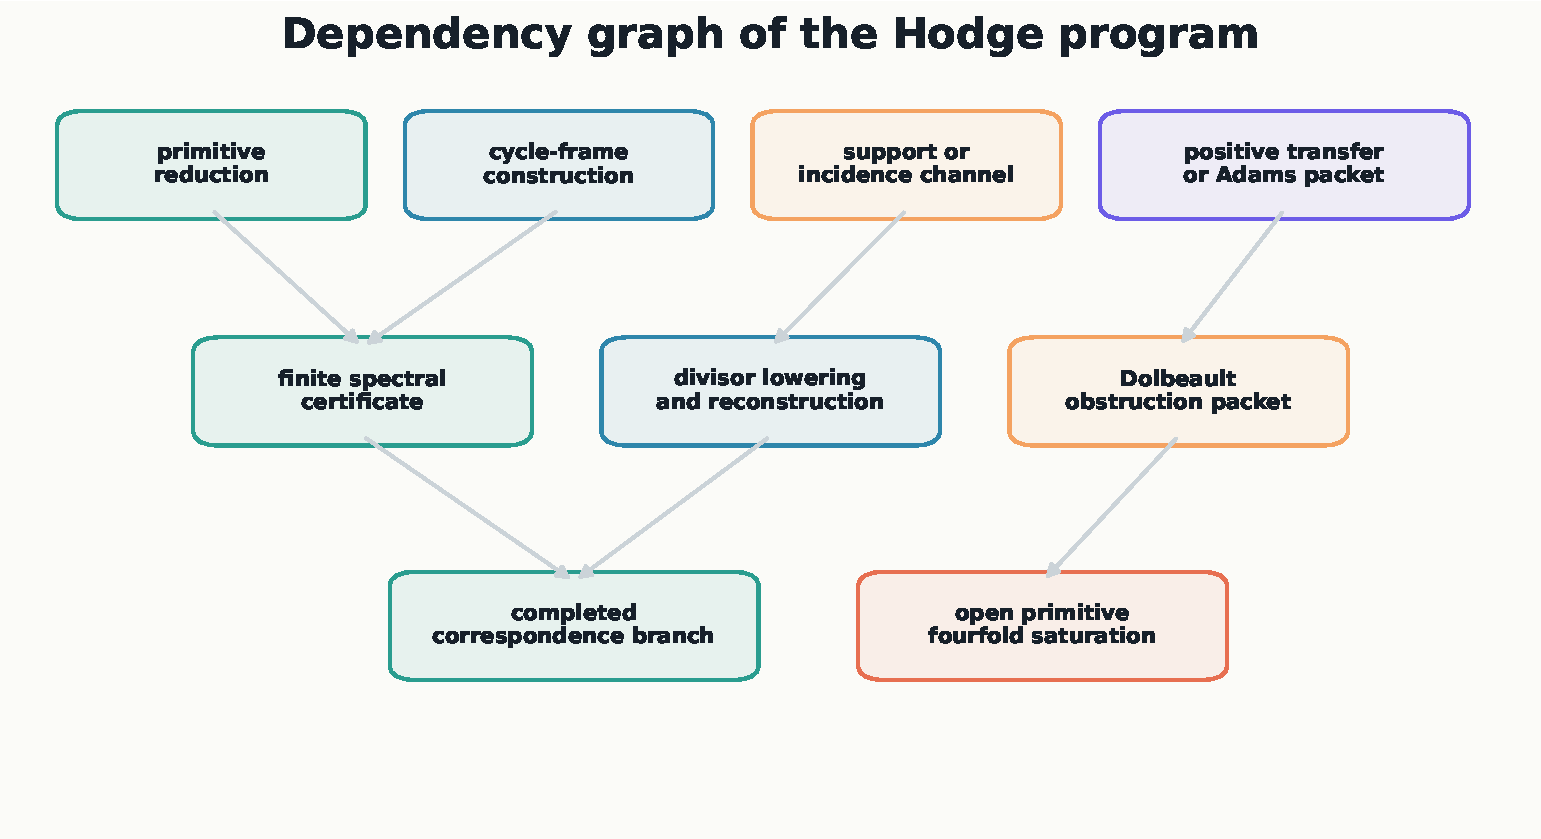
\includegraphics[width=0.92\textwidth]{29_hodge_dependency_graph.pdf}
\caption{Dependency graph. The correspondence branch is complete under an explicit invertible transfer, while primitive fourfold saturation remains open.}
\end{figure}

\begin{longtable}{p{0.40\textwidth}p{0.16\textwidth}p{0.34\textwidth}}
\caption{Atomic status ledger.}\label{tab:status}\\
\toprule
Statement & Status & Boundary \\
\midrule
\endfirsthead
\toprule
Statement & Status & Boundary \\
\midrule
\endhead
Master obstruction projector & Proved & Finite-dimensional linear algebra \\
Primitive Lefschetz reduction & Proved & Uses hard Lefschetz and algebraicity of the polarization \\
Degree-$2p$ coniveau identification & Proved & Rational coefficients and purity \\
Positive cycle-frame certificate & Proved & Requires an explicit finite cycle family \\
Exact degree polyphase assembly & Proved & Frame operators, not sums of span projectors \\
Finite saturation of bounded-degree spans & Proved & Non-effective degree bound \\
Support verification & Proved & Candidate support must already be supplied \\
Multiplicity reconstruction & Proved & Finite rational linear algebra \\
Divisor-lowering transfer theorem & Proved & Requires explicit algebraic correspondences and invertibility \\
Positive multi-channel criterion & Conditional & Algebraic realization of polarized adjoints is an extra hypothesis \\
Family propagation & Proved & Relative correspondences over a connected smooth base \\
Affine-paving branch & Proved & Classical localization argument \\
Projective bundle, blow-up, descent rules & Proved & Standard cohomological decompositions \\
Cubic and GM channels & Classical validation & Depend on established incidence Hodge isomorphisms \\
Adams degree projector & Proved & Rational topological K-theory \\
Range-packet nonlinear correction & Proved under hypotheses & Closed range, right inverse, and contraction bound \\
Vanishing of every harmonic obstruction packet & Open & Main analytic bridge \\
Primitive fourfold multi-incidence saturation & Open & Main geometric target \\
General rational Hodge conjecture & Open & No general cycle-generation theorem is claimed \\
\bottomrule
\end{longtable}

\begin{figure}[htbp]
\centering
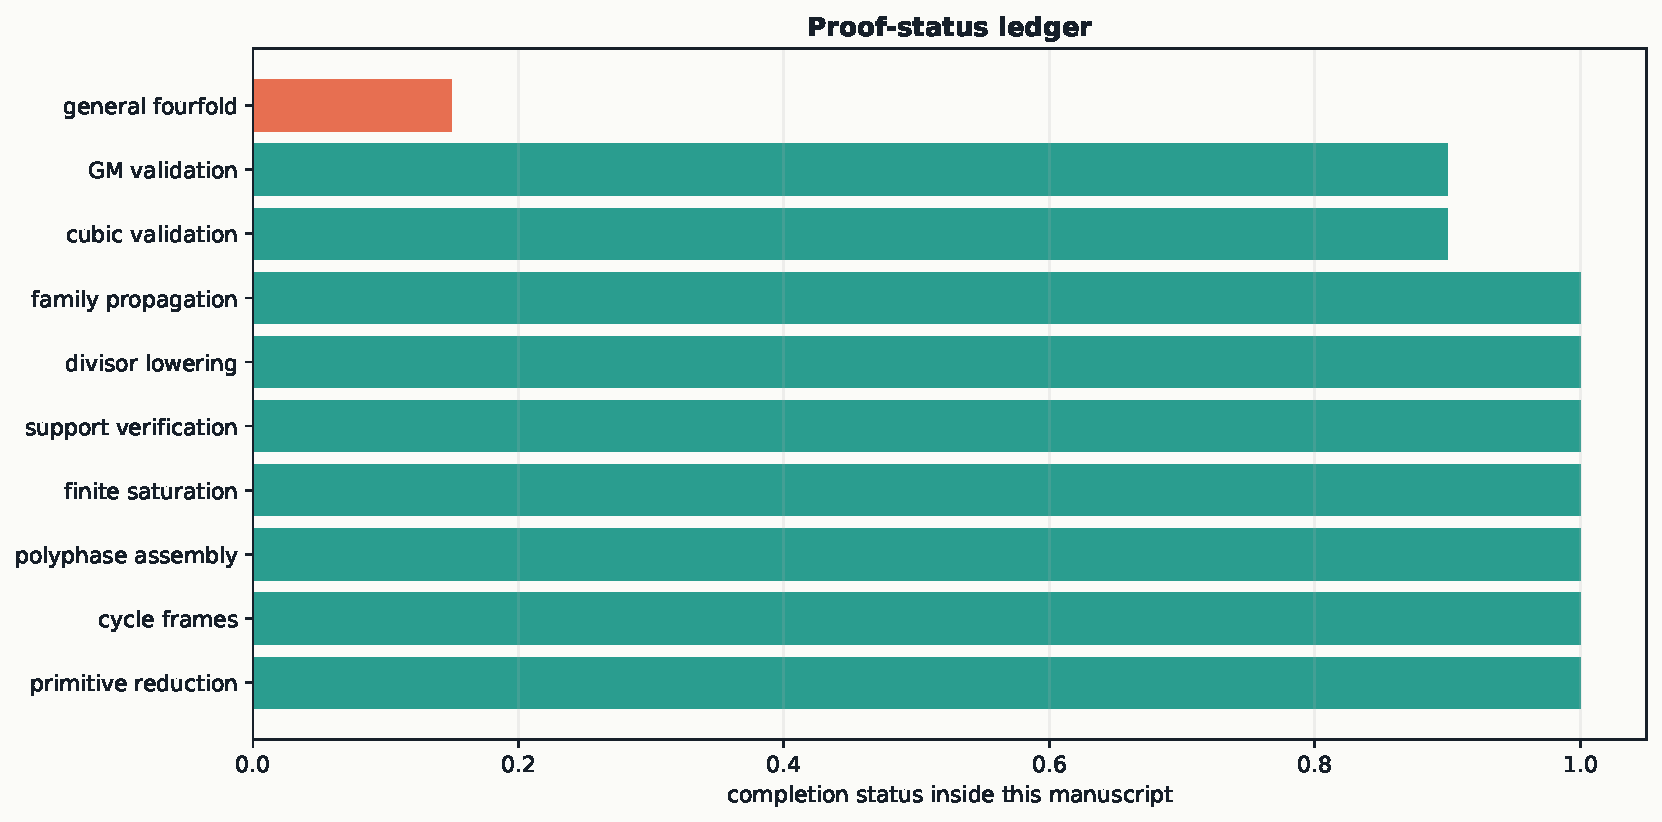
\includegraphics[width=0.78\textwidth]{32_status_ledger.pdf}
\caption{Visual status ledger for the finite core, validation cases, and open general target.}
\end{figure}

\chapter{The next realistic theorem: multi-incidence saturation}
Let $X$ be a special smooth projective fourfold. Construct algebraic lowering channels from families of subvarieties:
\[
A_{\mathrm{line}},
A_{\mathrm{conic}},
A_{\mathrm{plane}},
A_{\mathrm{exceptional}}.
\]
The exact target is
\[
\ker A_{\mathrm{line}}
\cap\ker A_{\mathrm{conic}}
\cap\ker A_{\mathrm{plane}}
\cap\ker A_{\mathrm{exceptional}}=\{0\}
\]
on primitive degree-four cohomology. Under algebraic adjoint hypotheses, equivalently prove
\[
T_{\mathrm{tot}}
=\sum_rA_r^\dagger A_r
\quad\text{satisfies}\quad
\lambda_{\min}(T_{\mathrm{tot}})>0.
\]

\begin{figure}[htbp]
\centering
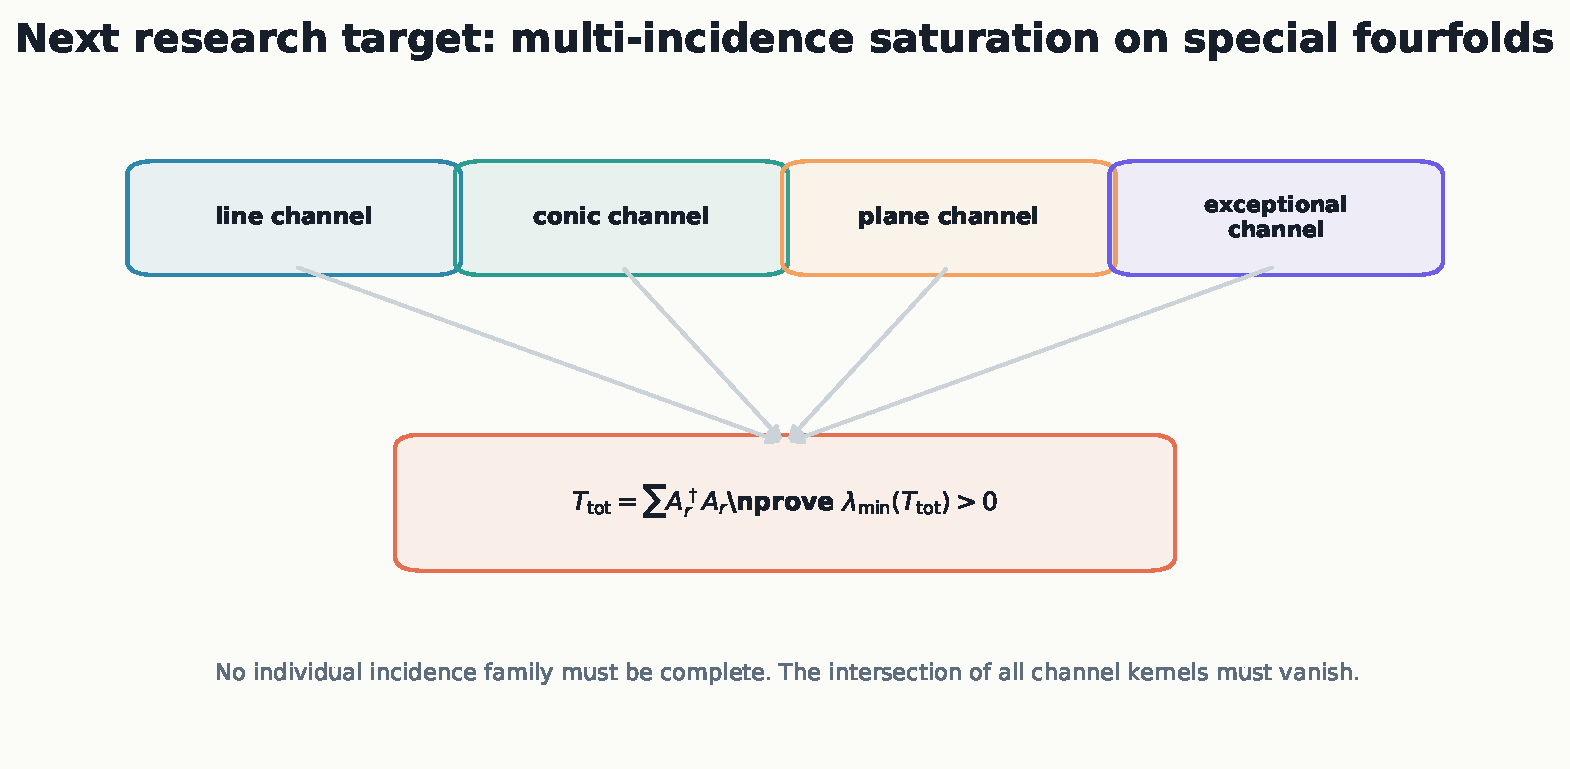
\includegraphics[width=0.86\textwidth]{30_multi_incidence_target.pdf}
\caption{The focused next theorem combines multiple incomplete incidence spaces into one positive saturating transfer.}
\end{figure}

\section{Why this target is realistic}
The problem is finite after the geometry is chosen:
\begin{enumerate}
\item compute the primitive cohomology representation and its symmetry decomposition
\item construct the incidence correspondences and their action
\item split the action into monodromy or symmetry packets
\item compute the joint kernel or positive Gram matrix over $\Q$
\item prove exact nonvanishing through rational rank, representation theory, or a dual certificate
\item invoke the divisor-lowering theorem to reconstruct cycles
\end{enumerate}
No single incidence family must be complete. Polyphase analysis permits separate geometric mechanisms to occupy separate primitive sectors.


\section{Three exact certificate forms}
Once the incidence channels have been constructed, the saturation statement admits three finite certificates. The geometric form is the kernel identity
\[
\bigcap_r\ker A_r=\{0\}.
\]
When algebraic correspondences realize the polarized adjoints, the equivalent positive form is
\[
\lambda_{\min}\left(\sum_rA_r^\dagger A_r\right)>0.
\]
In a rational basis, the final exact proof object is full column rank of the vertically stacked channel matrix. The kernel form explains the geometry, the positive form is stable for numerical scouting, and the rational rank form is appropriate for symbolic certification.

Two negative controls should accompany the proof. First, remove one channel at a time and recompute the joint kernel. If the kernel grows, the omitted incidence family is genuinely necessary. Second, refine a parent channel into geometric children and verify that their positive transfers sum exactly to the parent. This separates true packet coverage from accidental numerical invertibility.

A complete result should identify which primitive symmetry packets are detected by lines, conics, planes, or exceptional strata. The proof then becomes a finite occupancy statement: every primitive packet must be detected at least once. That structural description is more informative than a determinant alone and is the form most likely to propagate through families and degenerations.

\chapter{Computational and formal proof workflow}
Numerical experiments can scout candidate families but cannot replace an exact rank certificate. The intended pipeline is:
\[
\begin{aligned}
\text{exact incidence data}
&\longrightarrow \text{rational cohomology basis}
\longrightarrow \text{packet transfer matrices}\\
&\longrightarrow \text{rank or positivity certificate}
\longrightarrow \text{symbolic theorem proof}.
\end{aligned}
\]

\begin{figure}[htbp]
\centering
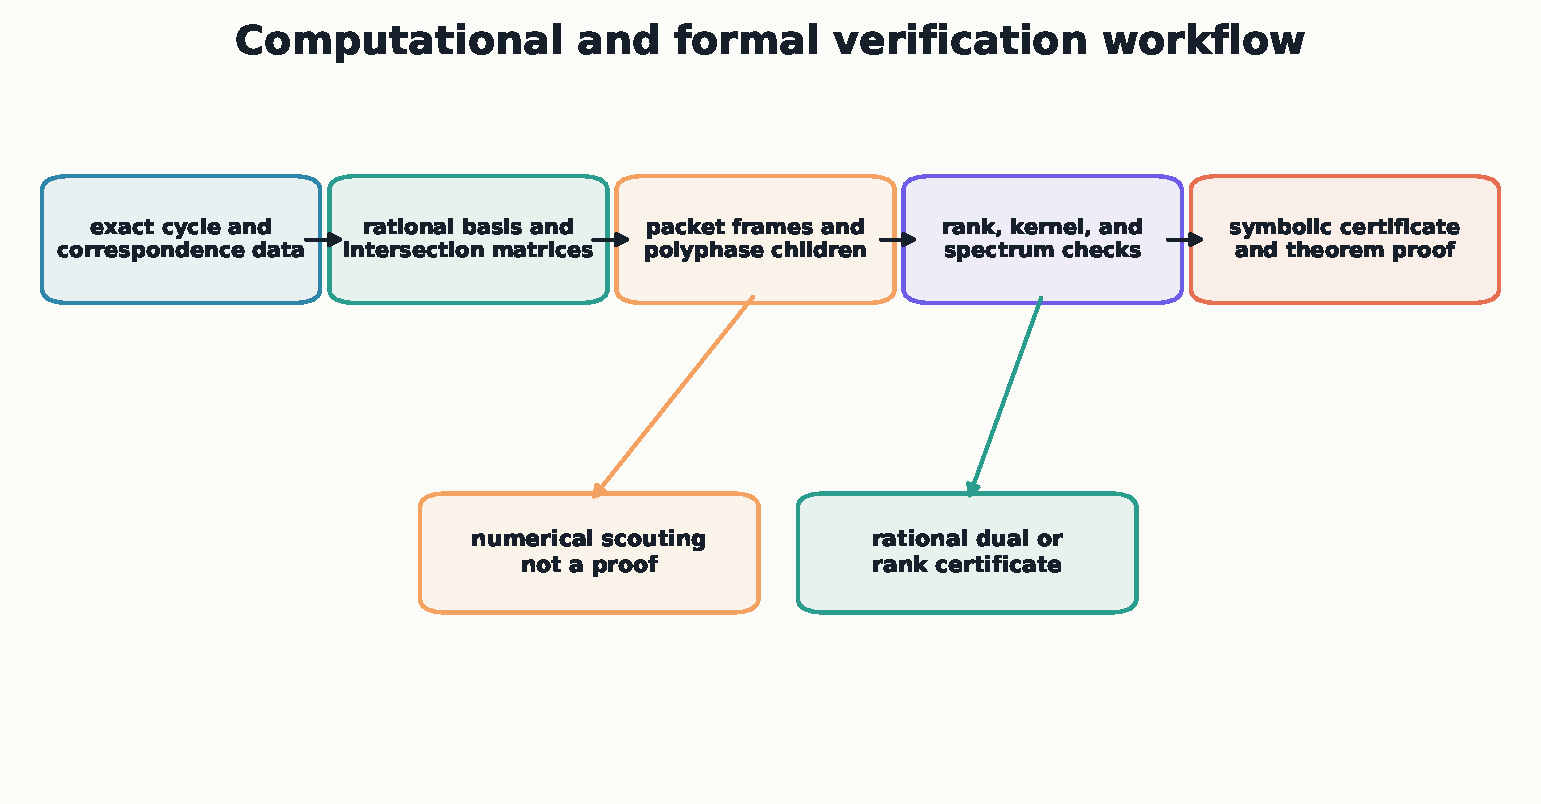
\includegraphics[width=0.9\textwidth]{31_verification_workflow.pdf}
\caption{Numerical scouting is separated from rational certification and formal theorem verification.}
\end{figure}

\section{Reproducible finite checks}
The accompanying Python generator produces all figures and runs eighteen independent finite checks covering:
\begin{itemize}
\item frame idempotency and range rank
\item positive Hodge Gram spectrum
\item exact modulo-$2$ and modulo-$4$ polyphase assembly
\item positive transfer rank and energy identities
\item Cayley-Hamilton inversion
\item contraction of the removable nonlinear packet
\item Adams projector idempotency and degree isolation
\item nilpotent trace blindness
\item support multiplicity recovery
\item finite rank stabilization
\end{itemize}
These tests verify the finite examples and implementation. They do not establish the open geometric saturation theorem.

\addcontentsline{toc}{part}{Appendices}

\appendix
\chapter{Formula registry}
\begin{longtable}{p{0.28\textwidth}p{0.62\textwidth}}
\toprule
Object & Formula \\
\midrule
Hodge packet & $\Hdg^p(X)=H^{2p}(X,\Q)\cap H^{p,p}(X)$ \\
Algebraic packet & $\Alg^p(X)=\im(\CH^p(X)_\Q\to H^{2p}(X,\Q))$ \\
Master obstruction & $\mathcal O_X^p=P_{\Hdg}^p-P_{\Alg}^p$ \\
Cycle frame & $S_D=C_DC_D^*=\sum_j|c_j\rangle\langle c_j|$ \\
Algebraic projector & $P_D=S_DS_D^\dagger$ \\
Polyphase parent & $S_{M,r}=\sum_{\ell=0}^{L-1}S_{LM,r+\ell M}$ \\
Support test & $j^*\alpha=0$ in $H^{2p}(X\setminus Z,\Q)$ \\
Transfer & $T=\sum_rB_rA_r$ \\
Positive transfer & $T=\sum_rA_r^\dagger A_r$ under algebraic-adjoint hypotheses \\
Adams projector & $e_p^{(m)}=\prod_{q\ne p}(\psi^m-m^qI)/(m^p-m^q)$ \\
Nonlinear defect & $F(a)=f+La+B(a,a)$ \\
Effective obstruction & $\Phi=\Pi(f+B(a_*,a_*))$ \\
Focused target & $\lambda_{\min}(\sum_rA_r^\dagger A_r)>0$ \\
\bottomrule
\end{longtable}

\chapter{Correspondence degree bookkeeping}
Let $X$ have dimension $n$ and $Y$ dimension $m$. A correspondence $\Gamma\in\CH^r(X\times Y)$ acts by
\[
\Gamma_*:H^i(X)\to H^{i+2(r-n)}(Y).
\]
To lower $H^{2p}(X)$ to $H^2(Y)$, choose $r=n-p+1$. To return $H^2(Y)$ to $H^{2p}(X)$, choose a correspondence of codimension $m+p-1$ on $Y\times X$. This bookkeeping is essential when inserting polarizations into transpose incidence correspondences.

\chapter{Verification table}
The machine-readable check table is distributed with the release. All eighteen checks are reproduced below. These checks validate the finite examples and code paths. They do not certify the open fourfold saturation theorem.
{\small
\begin{longtable}{p{0.43\textwidth}p{0.09\textwidth}p{0.22\textwidth}p{0.16\textwidth}}
\toprule
Check & Status & Value & Tolerance \\
\midrule
\endfirsthead
\toprule
Check & Status & Value & Tolerance \\
\midrule
\endhead
cycle frame projector idempotency & PASS & $2.11\times10^{-15}$ & $1\times10^{-12}$ \\
frame range rank & PASS & [8, 8] & equal \\
Hodge Gram positive & PASS & 2.2346 & $1\times10^{-5}$ \\
mod 2 assembly & PASS & $3.18\times10^{-15}$ & $1\times10^{-12}$ \\
mod 4 assembly & PASS & $4.47\times10^{-15}$ & $1\times10^{-12}$ \\
even child refinement & PASS & $1.29\times10^{-15}$ & $1\times10^{-12}$ \\
odd child refinement & PASS & $3.12\times10^{-15}$ & $1\times10^{-12}$ \\
positive transfer rank & PASS & [6, 6] & equal \\
positive transfer invertible & PASS & 1.5901 & $1\times10^{-6}$ \\
positive energy identity & PASS & $1.42\times10^{-14}$ & $1\times10^{-10}$ \\
Cayley Hamilton inverse & PASS & $5.81\times10^{-14}$ & $1\times10^{-10}$ \\
nonlinear contraction decreases & PASS & [0.010822, 0] & decrease \\
range equation residual & PASS & $8.51\times10^{-19}$ & $1\times10^{-10}$ \\
Adams projector idempotency & PASS & 0 & $1\times10^{-12}$ \\
Adams projector degree isolation & PASS & 0 & $1\times10^{-12}$ \\
nilpotent trace blindness & PASS & 0 & $1\times10^{-12}$ \\
support multiplicity reconstruction & PASS & $1.09\times10^{-14}$ & $1\times10^{-12}$ \\
finite rank stabilization & PASS & 6 & constant tail \\
\bottomrule
\end{longtable}
}


\chapter{Source and claim map}
The project uses three classes of input.
\begin{enumerate}
\item The internal projector-resolved seed calculus supplies exact reconstruction, positive packet assembly, obstruction packets, and polyphase parent-child semantics \cite{SeedI,SeedII,SeedIII}.
\item Classical Hodge theory supplies hard Lefschetz, Lefschetz $(1,1)$, purity, support exact sequences, and algebraic correspondences \cite{VoisinHodge,ClayHodge}.
\item Established incidence results supply the cubic and Gushel-Mukai validation channels \cite{BeauvilleDonagi,DebarreKuznetsov}.
\end{enumerate}
The new content of this manuscript is the unified packet organization, exact finite frame theorems, polyphase cycle assembly, the invertible divisor-lowering transfer criterion, the positive multi-channel formulation with its explicit hypothesis, and the focused multi-incidence research target. Historical priority for any theorem overlapping established correspondence or frame language must be audited before submission.

\backmatter
\chapter*{Conclusion}
\addcontentsline{toc}{chapter}{Conclusion}
The Hodge conjecture has been reduced to a collection of finite and geometric packets rather than treated as one opaque statement. The finite core is complete: primitive reduction, support verification, cycle-frame reconstruction, exact polyphase assembly, finite saturation, rational multiplicity recovery, invertible correspondence reconstruction, and several closure operations. The analytic range equation is also controlled under explicit Fredholm and smallness hypotheses.

\textbf{What is now exact.} For a fixed variety, a finite family of algebraic cycles gives a positive frame operator whose minimum Hodge-restricted eigenvalue is an exact saturation certificate. Degree-residue refinement assembles without assuming orthogonality. Bounded-degree cycle spans stabilize at a finite stage. A proposed support can be verified by restriction to its complement, after which rational multiplicities are recovered by intersection linear algebra. An invertible divisor-lowering correspondence transfer reconstructs every Hodge class in its domain from divisor classes on auxiliary varieties.

\textbf{What remains open.} None of the finite theorems proves that an arbitrary primitive rational Hodge class must enter one of the available cycle or correspondence channels. The analytic method removes the range component of the Dolbeault defect but leaves a finite obstruction packet. The geometric method supplies a finite saturation test but does not generate the required cycles for every fourfold. These are two coordinate descriptions of the same unresolved bridge.

\textbf{The immediate next experiment.} Choose a concrete family of special projective fourfolds with rich line, conic, plane, or exceptional incidence spaces. Compute their primitive cohomology and decompose it by symmetry. Construct every natural lowering channel and form the exact stacked rational transfer matrix. The first meaningful success is not a large numerical determinant. It is a proof that the joint kernel vanishes packet by packet, followed by divisor reconstruction through the transfer theorem.

The resulting research target is concise:
\[
\boxed{\text{Every primitive packet is detected by at least one algebraic incidence channel.}}
\]
A proof for a new family would be a genuine Hodge theorem for that family. A proof uniform across all fourfolds would close the first general open dimension. This manuscript establishes the infrastructure and the exact certificate, while keeping that final geometric generation statement visibly open.

\begin{thebibliography}{99}
\bibitem{ClayHodge}
Clay Mathematics Institute.
\newblock The Hodge Conjecture, Millennium Prize Problems.
\newblock \url{https://www.claymath.org/millennium/hodge-conjecture/}.

\bibitem{VoisinHodge}
C. Voisin.
\newblock \emph{Hodge Theory and Complex Algebraic Geometry I and II}.
\newblock Cambridge University Press, 2002--2003.

\bibitem{CDK}
E. Cattani, P. Deligne, and A. Kaplan.
\newblock On the locus of Hodge classes.
\newblock \emph{Journal of the American Mathematical Society}, 8:483--506, 1995.

\bibitem{AtiyahHirzebruch}
M. Atiyah and F. Hirzebruch.
\newblock Analytic cycles on complex manifolds.
\newblock \emph{Topology}, 1:25--45, 1962.

\bibitem{CharbonneauStern}
B. Charbonneau and M. Stern.
\newblock Asymptotic Hodge theory of vector bundles.
\newblock arXiv:1111.0591.

\bibitem{BeauvilleDonagi}
A. Beauville and R. Donagi.
\newblock La vari\'et\'e des droites d'une hypersurface cubique de dimension 4.
\newblock \emph{C. R. Acad. Sci. Paris S\'er. I Math.}, 301:703--706, 1985.

\bibitem{DebarreKuznetsov}
O. Debarre and A. Kuznetsov.
\newblock Gushel-Mukai varieties: linear spaces and periods.
\newblock \emph{Kyoto Journal of Mathematics}, 59:897--953, 2019.

\bibitem{SeedI}
Komorebi P.
\newblock \emph{Projector-Resolved Seed Calculus I: Typed Seeds, Operator Grammars, and Exact Reconstruction}.
\newblock Internal research manuscript, 2026.

\bibitem{SeedII}
Komorebi P.
\newblock \emph{Projector-Resolved Seed Calculus II: Polyphase Refinement, Weighted Transfer, and Dyadic-Odd Resolution}.
\newblock Internal research manuscript, 2026.

\bibitem{SeedIII}
Komorebi P.
\newblock \emph{Projector-Resolved Seed Calculus III: Nonlinear Operator Trees, Obstruction Packets, and Holonomy}.
\newblock Internal research manuscript, 2026.
\end{thebibliography}

\end{document}
